\documentclass[11pt,a4paper]{report}

\usepackage{lmodern}
\usepackage{algorithm}
\usepackage{url}
\usepackage{algpseudocode}
\usepackage{csquotes}
\usepackage[english]{babel}
\usepackage[T1]{fontenc}
\usepackage{graphicx}
\usepackage[11pt]{moresize}
\usepackage{amsmath}
\usepackage{amsthm}
\usepackage{amssymb}
\usepackage{hyperref}
\usepackage{physics}
\usepackage{scrextend}
\usepackage{wrapfig}
\usepackage{dsfont} % For the double-struck font
\usepackage[font=small,labelfont=bf,tableposition=top]{caption}
\usepackage[export]{adjustbox}
\usepackage[backend=bibtex,bibstyle=ieee,citestyle=numeric-comp]{biblatex}
\usepackage{float}
\usepackage{svg} % Include svg images
\svgsetup{inkscapelatex=false} % Avoid latex to overwrite the font

%\usepackage[sc]{mathpazo} % Use the Palatino font
%\linespread{1.05} % Line spacing - Palatino needs more space between lines

\newcommand{\vect}[1]{\boldsymbol{#1}}
\newcommand{\vettorec}[1]{\textrm{#1}}
\newcommand{\pscal}[2]{\langle \vettore{#1},\vettore{#2}\rangle}

\theoremstyle{definition}
\newtheorem{definizione}{Definizione}

\theoremstyle{plain}
\newtheorem{teorema}{Teorema}

\theoremstyle{plain}
\newtheorem{esempio}{Esempio}

\font\myfont=cmr12 at 40pt

\addbibresource{bibliography.bib}

 
\def\blankpage{%
      \clearpage%
      %\thispagestyle{empty}%
      %\addtocounter{page}{-1}%
      \null%
      \clearpage}

\begin{document}
    \pagenumbering{roman}
	\begin{titlepage}
    \begin{figure}
        \centering
        \includesvg[width=0.4\textwidth]{images/units_logo.svg}
    \end{figure}

    \begin{center}
        \LARGE{Università di Trieste\\}
        \vspace{5mm}
        \LARGE{Dipartimento di Matematica e Geoscienze\\}
        \vspace{5mm}
        \LARGE{Laurea Magistrale in Data Science \\ and Scientific Computing\\}

        \vspace{15mm}
        \HUGE{\bf Briscola Bot\\} \huge{\bf Mastering Briscola with model-free Deep Reinforcement Learning}

        \vspace{15mm}

    \end{center}

    \vspace{5mm}

    \begin{minipage}{0.47\textwidth}
        {\large{Relatore:}
            {\normalsize\vspace{3mm} \bf\\ \large{Prof: Antonio Celani}}}
        {\vspace{3mm} \large{\\Correlatore:}
            {\normalsize\vspace{3mm} \bf\\ \large{Emanuele Panizon}}}
    \end{minipage}
    \hfill
    \begin{minipage}{0.47\textwidth}\raggedleft
        {\large{Candidato:}{\normalsize\vspace{3mm} \bf\\ \large{Lorenzo Cavuoti}}}
    \end{minipage}

    \vspace{15mm}
    \centering{\large\bf{ANNO ACCADEMICO 2021/2022}}
\end{titlepage}
    \thispagestyle{empty}%
    \addtocounter{page}{-1}%
    \null%
    \clearpage
	\begin{center}
    \bf ABSTRACT
\end{center}
Recent developments in reinforcement learning demonstrate that it can be applied in a variety of domains, including card games. In this thesis, we present BriscolaBot, a reinforcement learning agent that learns to play the Italian card game of Briscola in a one-on-one setting. By utilizing the Proximal Policy Optimization (PPO) algorithm and training a deep neural network to learn the game's policy, our agent achieves performance comparable to that of an average human player. We also investigate the impact of various reward structures on the agent's learning process and identify potential areas of further improvement. To showcase the effectiveness of our agent, we provide a web-based version of the game where users can play against the trained agent, which can be accessed at \url{https://replit.com/@LorenzoCavuoti/BriscolaBot}. The code for the agent and the web-based game can be found in the GitHub repository \url{https://github.com/LetteraUnica/BriscolaBot}.
    \blankpage
	\chapter*{Ringraziamenti}

Ringrazio la mia famiglia che mi ha supportato durante tutti questi anni e mi ha dato la forza di proseguire. Ringrazio i miei amici, assieme a voi è sempre stato piacevole passare le serate. Ringrazio i miei compagni di corso, anche se purtroppo non ci siamo potuti vedere di persona per vari motivi, studiare assieme per gli esami è sempre stato divertente. Ringrazio il mio relatore Antonio Celani e correlatore Emanuele Panizon che hanno accolto questo progetto con entusiasmo e sono stati subito disponibili quando ne ho avuto bisogno.
	\blankpage

	\tableofcontents
    \blankpage
    \pagenumbering{arabic}
 	\chapter{Introduction}
Briscola is one of Italy's most popular card games \cite{briscola-wikipedia} and variations of it are also played in Portugal, Slovenia, Croatia and Montenegro. It can be played from two to six players. Briscola presents unique challenges for reinforcement learning due to its hidden information aspect. Unlike perfect information games like checkers, chess, and Go, established techniques cannot be easily applied to Briscola. Reinforcement learning in Briscola requires finding the best move under incomplete information about the game state, forcing the agent to make educated guesses about the cards held by other players.\\\\
In this thesis, we propose a new algorithm to learning to play Briscola in a one-on-one setting based on policy gradient methods with function approximation. Specifically, we adopt PPO with self-play, following the approach of OpenAI on Dota 2 \cite{open-ai-five}.\\
The policy gradient method is chosen due to its ability to learn any strategy, rather than being restricted to a deterministic one. This is crucial in learning to play Briscola, an imperfect information game, as a deterministic strategy will not necessarily result in the optimal play. To better understand this point, consider the game of poker. In a given situation, the best move is not always to check or to fold, but rather a combination of the two, in order to prevent the opponent from being able to determine what cards the agent is holding.\\\\
Our approach was able to learn how to play Briscola in a one-on-one setting in less than 20 minutes on a single computer, making it computationally efficient and easily replicable.\\
A web-based version of the game where the reader can play against the trained agent is available at \url{https://replit.com/@LorenzoCavuoti/BriscolaBot}.

\section{Game Theory}
Game theory is a branch of mathematics that focuses on the study of strategies for handling situations where the result of a player's action depends on the choices made by other participants.\\\\
Games like chess and Go are referred to as perfect information, zero-sum games. Perfect information means that all players have access to all information about the game state, while zero-sum means that what benefits one player harms the other, with no possibility for a win-win outcome. There are various techniques for finding or approximating the optimal strategy\footnote{The optimal strategy is the strategy that gives us the best win chance, assuming that the opponent plays perfectly.} in such games, like minimax search and Monte Carlo tree search (MCTS).

For instance, the Stockfish chess engine utilizes a form of minimax search called alpha-beta pruning, along with a heuristic evaluation function, to determine the best move \cite{stockfish}. Meanwhile, the Leela Chess Zero chess engine uses MCTS guided by a neural network \cite{lc0}.\\\\
In contrast, games like Briscola, poker, StarCraft II, Dota 2, and Kriegspiel are imperfect information, zero-sum games, imperfect information means that the game state is not fully observable. As a result, agents must make assumptions about the game state. In these games, the optimal play strategy is not deterministic, as a deterministic agent can be predictable and exploited by the opponent. When choosing the best move the agent must also take into account the information gained and the information that the agent might give to the opponent \cite{norvig-russell}.

Imperfect information games can still be solved by finding or approximating a Nash equilibrium. In a Nash equilibrium, no player has an incentive to change their strategy, as this will lead to a worse outcome for them. John Nash demonstrated in 1952 that every game with a finite number of players and actions has at least one Nash equilibrium \cite{nash-equilibrium-wikipedia}.


\section{Related work}
Existing approaches to learning Briscola can be broadly classified into three categories:
\begin{enumerate}
    \item \textbf{Rule based agents:} These agents use pre-determined, human-created rules to play the game. However, they lack the ability to adapt to new situations, as they are unable to learn from experience. The website \url{http://www.solitariconlecarte.it/briscola_2classica.htm} provides a rule based agent that plays Briscola.
    \item \textbf{Model-free agents:} These agents use model-free reinforcement learning techniques to learn the optimal strategy. They learn from experience through self-play or playing against other agents, such as a rule-based agent. At the time of writing, there are two known projects that use Deep Q-Learning (DQL) \cite{mnih2013playing} to learn Briscola. The first one \cite{fezriva-briscola-dqn} trains the DQL agent against a random agent, while the second \cite{alsora-deep-briscola-dqn} uses self-play to reach 90\% win rate against a random agent.
    \item \textbf{Search-based agents:} These agents employ Monte Carlo tree search (MCTS) to explore the game tree and find the best move. This approach has been successful in perfect information games like chess \cite{alphazero}, Go \cite{alphagozero} and backgammon \cite{td-gammon}, but requires a model of the environment to be effective. In the case of imperfect information games like Briscola, this model is not available as the strategies of other players are unknown. To overcome this, some approaches assume the other player will randomly play a card from the set of unseen cards \cite{Briscola-mcts-Playing-Algorithm}. A more flexible approach could involve learning a model of the other player to predict their moves, allowing the agent to adapt to their strategy.
\end{enumerate}
These approaches have also been combined, although not in Briscola. For instance, one of the earliest versions of AlphaGo \cite{alphago-fan} first learned Go strategies from professional human players, then refined the learned strategy using model-free reinforcement learning techniques. Lastly, it utilized Monte Carlo Tree Search (MCTS) to further enhance its performance during actual gameplay.\\\\
While developing our algorithm, we also looked at other card games such as poker, which has received significant attention over the years due to its popularity. In 2017, Libratus \cite{libratus} became the first program to defeat the world's best poker players by using the Counterfactual Regret Minimization (CFR) \cite{cfr} algorithm. CFR is an iterative method that converges to a Nash equilibrium in two-player zero-sum games like poker or Briscola. Recently, in 2020, ReBeL \cite{rebel} became the first program to beat the world's best poker players in full-table, not just one-on-one, no-limit Texas hold'em. ReBeL used a similar approach to CFR, but with the added use of deep neural networks to guide the algorithm, reducing the computational time required to reach the Nash equilibrium.

\section{Contributions}
The key contributions of this thesis are:
\begin{itemize}
    \item Presenting a novel algorithm for learning to play Briscola in a one-on-one setting using policy gradient methods with function approximation, based on PPO with self-play.
    \item Demonstrating that the algorithm achieves human-level play in less than 20 minutes of training on a standard 4-core computer, highlighting both its effectiveness and computational efficiency.
    \item Conducting ablation studies on the reward structure (comparing rewards based on points scored vs game outcome), evaluating the effectiveness of self-play, and exploring the impact of other hyperparameters.
    \item Developing a web-based version of the game where users can play Briscola against the trained agent, available at \url{https://replit.com/@LorenzoCavuoti/BriscolaBot}.
\end{itemize}

\section{Outline}
The rest of the thesis is organized as follows:
DA SCRIVERE
    \blankpage
    \chapter{Background}
When a human first plays a game, let it be chess, poker, Minecraft, CS:GO or any other game, it is not given any instructions on how to play. It is not told which moves are good and which are bad, maybe it doesn't even know the rules of the game. By interacting and playing the game, losing to some opponents and starting to beat others, the player gradually learns what moves are best in which situation and starts to understand the dynamics of the game. During all of this the player doesn't have any external feedback telling him which actions to perform in a given situation, but has to learn it by itself, by performing an action and experiencing the outcome. Learning from interaction is a foundational idea underlying nearly all theories of learning and intelligence \cite{sutton-barto}.\\\\
In this chapter we provide an overview of reinforcement learning. First we will discuss Markov Decision Processes (MDPs) that allow us to define an environment (for now we can think of an environment as a game) in mathematical terms, then we will discuss Dynamic Programming, that allows to solve exactly the reinforcement learning problem in case we know everything about the environment. Finally, we will see model-free methods, that allow us to learn even if we know nothing about the environment, these methods learn by interacting directly with the environment, obtaining experience and exploiting it to find the best actions to perform in any situation. This chapter is based on the first part of the Sutton and Barto book \cite{sutton-barto}

\section{Reinforcement Learning}
Reinforcement learning is the field of machine learning that tries to maximize a numerical reward signal. The agent is not said which actions to take, but instead must discover the actions that lead to the highest reward by trying them. Furthermore, actions do not only influence the immediate future reward but also the next situation and consequently subsequent rewards, so the agent must learn to balance immediate and future rewards.\\\\
Reinforcement learning differs from supervised learning because there is no external supervisor, which tells the agent which actions to perform in a given situation, instead the agent must discover the actions that lead to the highest reward by trying them. 
Reinforcement learning is also different from unsupervised learning, because even though both approaches do not need labels to learn from, their goal is different. In unsupervised learning the goal is to find structure in the data, while in reinforcement learning the goal is to maximize a reward signal.\\\\
One important aspect of reinforcement learning is the exploration-exploitation trade-off, which is not present in supervised or unsupervised learning. The agent must weigh the benefits of exploring new actions against the benefits of utilizing the best actions it has already discovered. A focus on exploration alone may lead to the discovery of the best actions, but with infrequent use, while a focus on exploitation alone may prevent the discovery of potentially better actions.

\section{Markov Decision Processes}
We can formalize the problem of learning from interaction to achieve a goal with Markov Decision Processes (MDPs). In the MPD framework the learner is called the agent, and the thing it interacts with is called the environment. The agent continually interacts with the environment by performing actions, on each action the environment changes state, and presents a new situation to the agent. The environment is also responsible to give the reward signal the agent must maximize \ref{fig:mdp}.
\begin{figure}[H]
    \centering
    \includesvg[width=0.6\textwidth]{images/mdp.svg}
    \caption{Illustration of the agent-environment interaction in a Markov Decision Process, image adapted from \cite{sutton-barto}.}
    \label{fig:mdp}
\end{figure}
More specifically, the agent and environment interact in discrete time steps ($t=0, 1, 2 \dots$). At each time step $t$ the agent receives an observation of the environment's state $S_t \in S$ and based on that chooses an action $A_t \in A$. In the next time step $t+1$ the agent receives from the environment a numerical reward $R_{t+1} \in R \in \mathbb{R}$ and a new observation $S_{t+1} \in S$ and so on. This generates a sequence of observations, actions and rewards, which we call trajectory: $S_0, A_0, R_1, S_1, A_1, R_2, \dots$.\\\\
In finite MDPs the set of states $S$, actions $A$ and rewards $R$ are finite, so the distribution of next state and reward, given the current state and action is well defined. Furthermore, the distribution of the random variables $R_t$ and $S_t$ follows the Markov property, depending only on the previous state and action, $P(S_{t+1}|S_t) = P(S_{t+1}|S_t, S_{t-1}, \dots, S_0)$.\\\\
We can formalize mathematically an MDP using the following notation:
\begin{itemize}
    \item $S$ is the set of states
    \item $A$ is the set of actions
    \item $R$ is the set of rewards
    \item $p(s', r | s, a)$ is the dynamics function, which describes the distribution of the next state $s'$ and reward $r$, given the current state $s$ and action $a$, defined as:
    \begin{equation}
        p(s', r | s, a) = \mathds{P}[S_{t+1} = s', R_{t+1} = r | S_t = s, A_t = a]
        \label{dynamics-function}
    \end{equation}
    \item $\gamma \in [0, 1]$ is the discount factor, which determines how much importance the agent gives to future rewards
\end{itemize}

\subsection{Reward}
The goal of the agent is formalized via a reward signal, given from the environment to the agent. At each time step the reward is a single number $R_t \in \mathbb{R}$. The agent goal is to maximize the total reward it receives over time.\\
For example if we want the agent to play a game, the reward signal can be the number of points the agent has scored. If we want the agent to learn to walk, the reward signal can be the distance the agent has traveled.\\
The reward signal is not a way of telling the agent how to do, if we were to do that the agent will accomplish side tasks without ever completing the main task that we want to be solved. For example in a racing game we might be tempted to give a reward whenever the car moves forward, but this will lead the agent to move forward and backward in a loop, without ever finishing the race. In fact, in this case finishing the race is the worst thing that could happen, because then the agent will stop receiving the reward signal.\\
The reward signal thus specifies what we want the agent to do, not how to do it.

\subsection{Episodic and Continuing Tasks}
We can divide the kinds of problems that reinforcement learning deals with in two classes: episodic problems and continuing ones, which can be both formalized with MDPs \ref{fig:episodic-continuing}.
\begin{figure}[H]
    \centering
    \includesvg[width=0.6\textwidth]{images/episodic-continuing.svg}
    \caption{Empty circles represent the states, while solid circles the actions state-action pairs. The numbers indicate the reward the agent receives if it goes through the corresponding transition. Left: Illustration of an episodic task, the terminal state $s_T$ is represented with a square. If the agent reaches the terminal state it can no longer receive any reward. Right: Illustration of a continuing task, when the agent reaches $s_2$ it comes back to $s_1$, receiving a reward of $r=1$ in the process, in this MPD the expected return with $\gamma = 1$ would be infinite as the sequence of rewards after the first state is always $1$.}
    \label{fig:episodic-continuing}
\end{figure}
In episodic tasks the agent interacts with the environment for a finite (yet random) number of time steps $T$, and then it reaches a terminal state, ending the episode. Examples of episodic tasks is the game of chess, as the episode ends when a player wins or a draw is made.\\
In continuing tasks, on the other hand, there is no clear notion of episode, as the agent interacts with the environment continually, potentially for an infinite number of time steps.\\
We can formalize both problems with MDPs, by defining the concept of terminal state: a terminal state is an absorbing state and corresponds to the end of the episode, when the agent reaches the terminal state it can no longer escape it and all future rewards are zero.\\


\subsection{Goal and Return}
In reinforcement learning we formalize the goal of an agent as the maximization of the expected return $\mathbb{E}[G_t]$, where the return, denoted as $G_t$ is the sum of all discounted rewards the agent receives in the future, starting from a given time step $t$:
\begin{equation}
    G_t = R_{t+1} + \gamma R_{t+2} + \gamma^2 R_{t+3} + \dots = \sum_{k=0}^{\infty} \gamma^k R_{t+k+1}
    \label{return}
\end{equation}
$\gamma \in [0, 1]$ is the discount factor and is used for two main reasons:
\begin{enumerate}
    \item $\gamma$ allows tuning how much importance the agent gives to future rewards, so we can make the agent more or less patient. If $\gamma = 0$ the agent will only consider the immediate reward $R_{t+1}$, while if $\gamma = 1$ the agent will consider all future rewards with the same importance.
    \item Allows the return to be used also in continuing tasks, because we can set $\gamma < 1$ and keep the sum from diverging.
\end{enumerate}
Returns of subsequent time steps are related to each other in an important way:
\begin{equation}
    G_t = R_{t+1} + \gamma G_{t+1}
    \label{return-recursive}
\end{equation}
Equation \eqref{return-recursive} is also called the one-step return.

\subsection{Policy and value functions}
A policy $\pi$ is a mapping from states to actions, which specifies what action the agent should take in a given state. The policy is formally defined as the probability of taking action $a$ in state $s$
\begin{equation}
    \pi(a | s) = \mathds{P}[A_t = a | S_t = s]
    \label{policy}
\end{equation}
Given a policy we can define a value function $v_{\pi}(s)$ associated to the policy, which gives us a measure of how good it is for the agent to be in a given state when following policy $\pi$. The value function is defined mathematically as the expected return starting from a state $s$ and then following policy $\pi$:
\begin{equation}
    v_{\pi}(s) = \mathds{E_{\pi}}[G_t | S_t = s] = \mathds{E_{\pi}}[\sum_{k=0}^{\infty} \gamma^k R_{t+k+1} | S_t = s]
    \label{value-function}
\end{equation}
We denote with $v_{\pi}(s)$ the value function of policy $\pi$.\\\\
Similarly, we can define the value of selecting an action $a$ in state $s$ under policy $\pi$, denoted $q_{\pi}(s, a)$, as the expected return starting from $s$, taking the action $a$ and then following policy $\pi$:
\begin{equation}
    q_{\pi}(s, a) = \mathds{E_{\pi}}[G_t | S_t = s, A_t = a] = \mathds{E_{\pi}}[\sum_{k=0}^{\infty} \gamma^k R_{t+k+1} | S_t = s, A_t = a]
    \label{action-value-function}
\end{equation}
We call $q_{\pi}(s, a)$ the action-value function of policy $\pi$.\\\\
In practice, it is also convenient to define the advantage, which is the difference between the value of taking action $a$ in state $s$ and the value of the state:
\begin{equation}
    A(s, a) = q_{\pi}(s, a) - v_{\pi}(s)
    \label{advantage}
\end{equation}
The advantage is a measure of how much better it is to take action $a$ in state $s$, with respect to the other possible actions in state $s$.\\

\subsection{Bellman Equation}
A fundamental property of the value function is that it satisfies a recursive relationship similar to the one of the return \eqref{return-recursive}:
\begin{equation}
    \begin{split}
        v_{\pi}(s) & = \mathds{E_{\pi}}[G_t | S_t = s] \\
        & = \mathds{E_{\pi}}[R_{t+1} + \gamma G_{t+1} | S_t = s] \\
        & = \sum_a \pi(a | s) \sum_{s', r} p(s', r | s, a) (r + \gamma v_{\pi}(s'))
    \end{split}
    \label{bellman-equation}
\end{equation}
We call equation \eqref{bellman-equation} the Bellman equation for $v_{\pi}$. The Bellman equation expresses the relationship between the value of current state $s$ and the value of successive states $s'$. It tells us that the value of each state must equal the value of the next state plus the reward expected along the way. The Bellman equation forms the basis to compute or approximate $v_{\pi}$ which we will see in the next  section.\\\\
It is also possible to define the Bellman equation for the action-value function:
\begin{equation}
    \begin{split}
        q_{\pi}(s, a) & = \mathds{E}[G_t | S_t = s, A_t = a] \\
        & = \mathds{E}[R_{t+1} + \gamma G_{t+1} | S_t = s, A_t = a] \\
        & = \sum_{s', r} p(s', r | s, a) (r + \gamma v(s')) \\
        & = \sum_{s', r} p(s', r | s, a) (r + \gamma \sum_{a'} \pi(a' | s') q_{\pi}(s', a'))
    \end{split}
    \label{bellman-equation-action-value}
\end{equation}
Where in the last step we used the relationship $v_{\pi}(s) = \sum_a \pi(a | s) q_{\pi}(s, a)$ between the value function and action-value function.\\\\

\subsection{Optimal policy and value function}
Solving a reinforcement learning problem means finding a policy that achieves a high return. To accomplish this we first need to define an ordering over policies. We define that policy $\pi$ is better than policy $\pi'$ if the expected return is higher for $\pi$ than for $\pi'$.
\begin{equation}
    \pi \geq \pi' \iff v_{\pi}(s) \geq v_{\pi'}(s) \quad \forall s \in S
    \label{policy-ordering}
\end{equation}
This way we can define the optimal policy as the policy that is at least better or equal to all other policies.
\begin{equation}
    \pi^* \geq \pi' \quad \forall \pi'
    \label{optimal-policy}
\end{equation}
Although there may be more than one optimal policy, all of them will have the same value-function $v_*$, so we can denote all the optimal policies with $\pi^*$.
We define the optimal state-value function $v_*$ as:
\begin{equation}
    v_*(s) = \max_{\pi} v_{\pi}(s) \quad \forall s \in S
    \label{optimal-value-function}
\end{equation}
Which is the value function that achieves the maximum return from all states $s$. We can also define the optimal action-value function $q_*$ as:
\begin{equation}
    q_*(s, a) = \max_{\pi} q_{\pi}(s, a) \quad \forall s \in S, \forall a \in A
    \label{optimal-action-value-function}
\end{equation}
This function gives the expected return for taking action $a$ in state $s$ and then following policy $\pi^*$.\\\\
Another property of the optimal state-value function is that it satisfies a special form of the Bellman equation \eqref{bellman-equation}, called the Bellman optimality equation:
\begin{equation}
    \begin{split}
        v_{*}(s) & = \max_a q_*(s, a) \\
        & = \max_a \mathds{E_{\pi^*}}[G_t | S_t = s, A_t = a] \\
        & = \max_a \sum_{s', r} p(s', r | s, a) (r + \gamma v_*(s'))
    \end{split}
    \label{bellman-optimality-equation}
\end{equation}
Note that in the final statement we didn't specify any policy, this is because we assume to be following an optimal policy, which is the one that always selects the best action $a_* = \arg \max_a' q_*(s, a') \; \forall s \in S$.
Analogously, we can define the Bellman optimality equation for the action-value function:
\begin{equation}
    \begin{split}
        q_{*}(s, a) & = \mathds{E_{\pi^*}}[G_t | S_t = s, A_t = a] \\
        & = \sum_{s', r} p(s', r | s, a) (r + \gamma \max_{a'} q_*(s', a'))
    \end{split}
    \label{bellman-optimality-equation-action-value}
\end{equation}
Intuitively, the Bellman optimality equation expresses the fact that the value of a state under an optimal policy must equal the expected return for the best action from that state.\\
In the next sections we will see how to solve the Bellman optimality equation both when we have a model of the environment \eqref{dynamics-function} and when we don't.

\section{Dynamic Programming}
Dynamic programming is a technique that allows us to solve the Bellman optimality equation \eqref{bellman-optimality-equation}, finding the optimal policy $\pi_*$ and value function $v_*$ given a perfect model of the environment, that is, we completely know the dynamics function $p(s', r | s, a)$.
We can split the problem of finding a solution to the Bellman optimality equation into two subproblems:
\begin{enumerate}
    \item \textbf{Policy evaluation}: Given a policy $\pi$, find its value function $v_{\pi}$.
    \item \textbf{Policy improvement}: Given the value function $v_{\pi}$, find a better policy $\pi'$.
\end{enumerate}

\subsection{Policy evaluation}
A simple way to evaluate a policy $\pi$ would be to solve the linear system of equations described by the Bellman equation \eqref{bellman-equation}. This could be done with any linear system solution method available in the literature, however, in reinforcement learning iterative solution methods are most suitable.
\begin{algorithm}[H]
    \caption{Policy evaluation}
    \label{alg:policy-evaluation}
    \begin{algorithmic}[1]
        \Require A policy $\pi$, a model $p$, a discount factor $\gamma$, a threshold $\theta$
        \State Initialize a candidate value function $\hat{v}_{\pi}$
        \While{True}
            \State $\hat{v}'_{\pi} = \hat{v}_{\pi}$
            \For{$s \in S$}
                \State $\hat{v}'_{\pi}(s) = \sum_a \pi(a | s) \sum_{s', r} p(s', r | s, a) (r + \gamma \hat{v}_{\pi}(s'))$
            \EndFor
            \If{$| \hat{v}'_{\pi}(s) - \hat{v}_{\pi}(s) | < \theta$}
                \State \textbf{return} $\hat{v}_{\pi}$
            \EndIf
        \EndWhile
    \end{algorithmic}
\end{algorithm}
Algorithm \ref{alg:policy-evaluation} is called the iteative policy evaluation algorithm and is guaranteed to always converge to the true value function $v_{\pi}$ with an error below the threshold $\theta$ if $\gamma < 1$, or if $\gamma = 1$ only if termination is guaranteed from all states under the policy $\pi$.\\
This can be proven mathematically by noting that the operator $B_{\pi}(v_{\pi}) = \sum_a \pi(a | s) \sum_{s', r} p(s', r | s, a) (r + \gamma v_{\pi}(s'))$ is contracting, which means that the solution is both unique and is reached no matter how we initialize the value function $\hat{v}_{\pi}$.\\\\
In algorithm \ref{alg:policy-evaluation} we used an additional array to store the updated value function $\hat{v}'_{\pi}$, however, this is not required, as the algorithm will converge regardless of how we perform the updates, that is, we could have used only one array $\hat{v}_{\pi}$ and performed the update in line $5$ in-place:\\
$\hat{v}_{\pi}(s) = \sum_a \pi(a | s) \sum_{s', r} p(s', r | s, a) (r + \gamma \hat{v}_{\pi}(s'))$\\
In practice, the in-place algorithm usually converges faster than the two-array version because it uses updated values as soon as they are available.

\subsection{Policy improvement}
Our reason for computing the value function for a policy is to help find better policies. A simple improved version of $\pi$ is a policy that in state $s'$ takes the action that maximizes $q_{\pi}(s', a)$. This policy will be equal to $\pi$ in all states $s \neq s'$ but will be better in state $s'$, so $\pi' \geq \pi$.\\
We can take this idea further, by defining $\pi'$ as the policy that takes the greedy action with respect to $q_{\pi}(s, a)$ in all states, with ties broken evenly. This policy is called the greedy policy and is defined as:
\begin{equation}
    \pi'(a | s) = \arg \max_a q_{\pi}(s, a) = \arg \max_a \sum_{s', r} p(s', r | s, a) (r + \gamma v_{\pi}(s'))
    \label{greedy-policy}
\end{equation}
The greedy policy always takes the action that looks best in the short term with just one-step look ahead, according to $v_{\pi}$. It can be shown that the greedy policy is always better or equal to $\pi$ due to the policy improvement theorem, demonstrated on page 78 of the Sutton and Barto's book \cite{sutton-barto}.

\subsection{Policy iteration}
A simple way to find the optimal policy is to iterate the policy evaluation and policy improvement steps until the policy doesn't change anymore. This process is guaranteed to converge to the optimal policy and value function with the same conditions that apply to the policy evaluation algorithm \ref{alg:policy-evaluation}, that is: convergence is guaranteed to the true value function $v_{\pi}$ with an error below the threshold $\theta$ if $\gamma < 1$, or if $\gamma = 1$ and the task is episodic.
\begin{algorithm}[H]
    \caption{Policy iteration}
    \label{alg:policy-iteration}
    \begin{algorithmic}[1]
        \Require A model $p$, a discount factor $\gamma$, a threshold $\theta$
        \State Initialize a policy $\pi$
        \While{True}
            \State $v_{\pi} = \mathrm{Policy \; evaluation} (\pi, p, \gamma, \theta)$ \Comment{Algorithm \ref{alg:policy-evaluation}}
            \State $\pi' = \arg \max_a \sum_{s', r} p(s', r | s, a) (r + \gamma v_{\pi}(s'))$ \Comment{Policy improvement}
            \If{$\pi' = \pi$}
                \State \textbf{return} $\pi, v_{\pi}$
            \EndIf
        \EndWhile
    \end{algorithmic}
\end{algorithm}
Algorithm \ref{alg:policy-iteration} is called the policy iteration algorithm. The algorithm iterates the policy evaluation and policy improvement steps until the policy doesn't change anymore.

\subsection{Value iteration}
The drawback of the policy iteration algorithm \ref{alg:policy-iteration} is that it requires an entire policy evaluation for each policy improvement step, requiring multiple sweeps over the state space. In practice, however, we can stop before policy evaluation finished without losing any of the convergence properties of policy iteration \ref{alg:policy-iteration}. One important special case is when policy evaluation is stopped after just one sweep, using the update:
\begin{equation}
    v_{k+1}(s) = \max_a \sum_{s', r} p(s', r | s, a) (r + \gamma v_k(s'))
    \label{value-iteration-update}
\end{equation}
This update is called the value iteration update and combines one pass of policy evaluation and policy improvement into one, requiring only 1 sweep over the state space. The update \eqref{value-iteration-update} is similar to the policy evaluation update \eqref{bellman-equation} except that we are using the maximum instead of the expectation.
\begin{algorithm}[H]
    \caption{Value iteration}
    \label{alg:value-iteration}
    \begin{algorithmic}[1]
        \Require A model $p$, a discount factor $\gamma$, a threshold $\theta$
        \State Initialize a value function $v_{0}$
        \While{True}
            \State $v_{k+1} = v_k$
            \For{$s \in S$}
                \State $v_{k+1}(s) = \max_a \sum_{s', r} p(s', r | s, a) (r + \gamma v_k(s'))$
            \EndFor
            \If{$| v_{k+1}(s) - v_k(s) | < \theta$}
                \State \textbf{return} $v_{k+1}$
            \EndIf
        \EndWhile
    \end{algorithmic}
\end{algorithm}
Algorithm \ref{alg:value-iteration} usually converges faster than policy iteration \ref{alg:policy-iteration}. Furthermore, like the policy iteration algorithm, this algorithm converges even if we perform all updates in place, without needing to keep in memory both $v_{k+1}$ and $v_k$, thus reducing memory requirements.\\\\
The value iteration algorithm \ref{alg:value-iteration} has a limitation in that it necessitates a complete examination of the entire state space, which can be an issue if the state space is large. However, the algorithm is still guaranteed to converge to the optimal value function even if updates are performed on certain states more frequently than others, as long as we continue to update all the states. These algorithms are called asynchronous DP algorithms because they update the values of the states in asynchronous fashion.

\subsection{Generalized policy iteration}
\begin{wrapfigure}{r}{0.4\textwidth}
    \centering
    \includesvg[width=0.3\textwidth]{images/GPI.svg}
    \caption{Generalized policy iteration loop. Image adapted from \cite{sutton-barto}.}
    \label{fig:gpi}
\end{wrapfigure} 
We can view both the policy iteration algorithm \ref{alg:policy-iteration} and the value iteration algorithm \ref{alg:value-iteration} as special cases of a more general process referred to as generalized policy iteration (GPI). Almost all RL algorithms are described by this process where the policy is improved towards the value function and vice-versa, as shown in figure \ref{fig:gpi}. This loop ends only when we reach a policy that is greedy with respect to its own value function, which implies that the value function satisfies the Bellman optimality equation \eqref{bellman-optimality-equation}.\\
Another way to see the process is in terms of two different goals, the two converging lines represented in figure \ref{fig:gpi2}. The first goal is to compute the value function of a policy $v=v_{\pi}$, which is achieved by policy evaluation. The second goal is to make the policy greedy with respect to its own value function $\pi=\mathrm{greedy}(v)$, which is achieved by policy improvement. The two goals are complementary and the process converges to the optimal value function when the two goals are achieved simultaneously.
\begin{figure}[H]
    \centering
    \includesvg[width=\textwidth]{images/policy-and-value-iteration-gpi.svg}
    \caption{Another way to see generalized policy iteration. Left: policy iteration with full policy evaluation at each step. Right: policy iteration with truncated policy evaluation at each step. Image adapted from \cite{sutton-barto}.}
    \label{fig:gpi2}
\end{figure}

\section{Monte Carlo methods}
Monte Carlo methods are a class of algorithms that learn directly from experience, without the need for a model of the environment. The main idea is to estimate the value function $v_{\pi}$ by averaging the returns $G_t$ following each state. These methods can only be applied to episodic tasks because we update the value function using $G_t$, which is only available after an episode has finished.\\
As with dynamic programming we can split the problem of finding the optimal policy into two parts.
\begin{enumerate}
    \item Monte Carlo prediction: estimate the value function $v_{\pi}$ corresponding to a given policy $\pi$
    \item Monte Carlo control: find the optimal policy $\pi^*$
\end{enumerate}

\subsection{Monte Carlo prediction}
Suppose we have a policy $\pi$, and we want to estimate the value function $v_{\pi}$ given a set of episodes obtained by following policy $\pi$, and passing through state $s$ at time $t$. We call each occurrence of state $s$ in an episode a visit to $s$. Of course, $s$ may be visited multiple times in the same episode, so we can call the first time $s$ is visited in an episode the first visit to $s$. We can then identify two main methods to perform Monte Carlo policy evaluation:
\begin{enumerate}
    \item First-visit MC method: estimate $v_{\pi}(s)$ as the average of the returns following first visits to $s$.
    \item Every-visit MC method: estimate $v_{\pi}(s)$ as the average of the returns following all visits to $s$.
\end{enumerate}
For example, in the first visit case we estimate the value function $v_{\pi}$ as follows:
\begin{equation}
    \begin{split}
    v_{\pi}(s) & = \mathds{E}_{\pi}(G_t | S_t = s)\\
    & = \frac{1}{N} \sum_{i=1}^N G_t^{(i)}\\
    & = \frac{1}{N} \sum_{i=1}^N \sum_{t'=t}^{T} \gamma^{t'} R_{t'+1}^{(i)}
    \end{split}
    \label{mc-prediction}
\end{equation}
Where $G_t^{(i)}$ is the return after visiting state $s$ in the $i$-th episode, $N$ is the number of episodes and $T$ is the episode length.\\
As the number of visits to state $s$ increases, both first-visit and every-visit Monte Carlo methods converge to $v_{\pi}(s)$. However, the two methods have different theoretical characteristics. First-visit MC provides independent and identically distributed estimates of $v_{\pi}(s)$, whereas every-visit MC does not. Despite its less straightforward nature, every-visit MC still maintains the same convergence properties as first-visit MC.\\\\
Monte Carlo methods can be utilized to estimate the action-value function $q_{\pi}(s, a)$ as well, which is critical for control tasks. The concept of visits is redefined to apply to state-action pairs, rather than states alone. A state-action pair $(s, a)$ is considered visited if action $a$ was selected while in state $s$.

\subsection{Monte Carlo control}
In the control problem, MC methods draw from the idea of generalized policy iteration (GPI) already presented: alternating between policy evaluation and policy improvement.\\
In the policy evaluation step we estimate the action-value function $q_{\pi}$ using the first visit or every visit MC method. However, we need to ensure that all states will be visited, to accomplish this we can generate the episodes with exploring starts, that is, all episodes begin with state-action pairs randomly selected to cover all possibilities.\\
The policy improvement step, on the other hand, is performed by greedily selecting the action that maximizes the action-value function \eqref{mc-policy-improvement}, which is the same as selecting the action that maximizes the expected return.
\begin{equation}
    \pi'(s) = \arg \max_a q_{\pi}(s, a)
    \label{mc-policy-improvement}
\end{equation}
A major problem with this approach is the exploring starts assumption, because, if we are not given a model of the environment, we cannot know all state-action pairs beforehand, and even if we did, we would still need to generate many episodes to ensure that all state-action pairs are visited. Without exploring starts, the only general way to ensure that all actions are selected infinitely often is for the agent to continue to select them. This can be done in two ways:
\begin{enumerate}
    \item We can use a different policy to generate the episodes, a behavioral policy, different from the one we are trying to improve, the target policy. This is called off-policy learning.
    \item We can avoid making the policy completely greedy like in equation \eqref{mc-policy-improvement} and instead use an $\epsilon$-soft policy, which is a policy that is not completely greedy, but gives at least probability $\epsilon / |A|$ to each action. An example of such policy is the $\epsilon$-greedy policy, defined as follows:
    \begin{equation}
        \pi(a|s) = \begin{cases}
            1 - \epsilon + \frac{\epsilon}{|A|} & \text{if } a = \mathrm{argmax}_{a'} q_{\pi}(s, a') \\
            \frac{\epsilon}{|A|} & \text{otherwise}
        \end{cases}
        \label{epsilon-greedy-policy}
    \end{equation}
\end{enumerate}

\section{Temporal-Difference learning}
Temporal-difference learning, also called TD-Learning, is a class of algorithms that combine both Monte Carlo and dynamic programming ideas. Like Monte Carlo, TD-learning methods learn directly from experience, not requiring a model of the environment, and like DP it updates the value function with already learned estimates, using a technique known as bootstrapping. This allows TD methods to be also applied to continuing tasks because they can update the value of a state as soon as new information is available.\\
Like we did with Monte Carlo methods, we first focus on the prediction problem, then the control one.

\subsection{TD prediction}
TD prediction uses the one-step return, represented as $G_{t:t+1} = R_{t+1} + \gamma G_{t+1}$ (as defined in equation \eqref{return-recursive}), rather than the full return (defined in equation \eqref{return}) to estimate the value function. To obtain the expected return, which is needed to estimate the value function, we take the expected value of the recursive formula.
\begin{equation}
    \begin{split}
        v_{\pi}(s) & = \mathds{E}_{\pi}(G_t | S_t = s) \\
        & = \mathds{E}_{\pi}(R_{t+1} + \gamma G_{t+1} | S_t = s)\\
    \end{split}
    \label{td0-expected-return}
\end{equation}
This expectation \eqref{td0-expected-return} can be directly estimated by sampling episodes according to the policy $\pi$. The value function $v_{\pi}$ is then updated as follows:
\begin{equation}
    V(S_t) = V(S_t) + \alpha (R_t + V(S_t) - V(S_{t+1}))
    \label{td0-update}
\end{equation}
Where we introduced a parameter $\alpha$ which is the learning rate of the algorithm, the learning rate controls how much the new estimate of the value gathered in the episode should count with respect to the previous value estimate $V(S_t)$.\\
Finally, the quantity in parentheses $\delta = R_t + V(S_t) - V(S_{t+1})$ is known as the TD error, and measures the difference between the estimated value of the current state $V(S_t)$ and the better estimate $R_t + V(S_{t+1})$, given by the episode.\\
Updating the value function in this way \eqref{td0-update} introduces bias in the value estimate, however, this also reduces the variance, which is why TD methods usually learn faster Monte Carlo methods.

\subsection{TD control}
In TD control we need to estimate the action-value function $q_{\pi}(s, a)$, rather than a state-value function. There are three main methods to do so, Sarsa, Expected Sarsa and Q-learning.

\subsubsection{Sarsa}
Sarsa is the simplest of the three, it is an on-policy TD control method that uses the following update rule to estimate the action-value function:
\begin{equation}
    Q(S_t, A_t) = Q(S_t, A_t) + \alpha (R_{t+1} + \gamma Q(S_{t+1}, A_{t+1}) - Q(S_t, A_t))
    \label{Sarsa-update}
\end{equation}
The method is called Sarsa because in state $S_t$ it selects action $A_t$, then observes reward $R_{t+1}$ and next state $S_{t+1}$, finally it selects the next action $A_{t+1}$.\\
In Sarsa $Q(S_{t+1}, A_{t+1})$ is a sample of the value of the next state $V(S_{t+1})$, because the next action $A_{t+1}$ is selected according to policy $\pi$.
\begin{equation*}
    \begin{split}
        v_{\pi}(s') & = \sum_a{q(s', a) \pi(a | s')} \\
        & = \mathds{E}_{\pi}(Q(S_{t+1}, A_{t+1}) | S_{t+1} = s')
    \end{split}
\end{equation*}

\subsubsection{Expected Sarsa}
Expected Sarsa, estimates the value of the next state by using directly its expected value $V(S_{t+1})$. The update rule of expected Sarsa is thus the following.
\begin{equation}
    \begin{split}
        Q(S_t, A_t) & = Q(S_t, A_t) + \alpha (R_{t+1} + \gamma V(S_{t+1}) - Q(S_t, A_t)) \\
        & = Q(S_t, A_t) + \alpha (R_{t+1} + \gamma \sum_a{Q(S_{t+1}, a) \pi(a | S_{t+1})} - Q(S_t, A_t))
    \end{split}
    \label{expected-Sarsa-update}
\end{equation}
This update reduces the variance of the value estimate, but it also increases its computational cost, because to compute the value of the next state we must sum over all actions, $V(S_{t+1}) = \sum_a{Q(S_{t+1}, a) \pi(a | S_{t+1})}$, which can be computationally expensive when the number of actions is high.

\subsubsection{Q-learning}
Q-learning is an off-policy TD control method, that uses the following update rule to estimate the action-value function:
\begin{equation}
    Q(S_t, A_t) = Q(S_t, A_t) + \alpha (R_{t+1} + \gamma \max_a{Q(S_{t+1}, a)} - Q(S_t, A_t))
    \label{Q-learning-update}
\end{equation}
Q-learning assumes that the next action $A_{t+1}$ is selected according to a greedy policy with respect to the action-value function $Q(S_{t+1}, a)$. In this algorithm, the learned action-value function directly approximates the optimal action-value function $q_*$, independently of the policy being followed. However, the policy $\pi$ still has an important effect because it determines which state-action pairs are visited and is thus called the behavioral policy.

\section{$n$-step methods}
$n$-step methods merge the gap between MC and TD methods, so that one can shift from one to the other smoothly. This is important because the best method for a given problem is often intermediate between these two extremes figure \ref{fig:n-step-comparison}.\\\\
$n$-step methods estimate the value function using the $n$-step return, which is the sum of the rewards obtained in the next $n$ steps, plus the value of the state reached after $n$ steps.\\
\begin{equation}
    G_{t:t+n} = R_{t+1} + \gamma R_{t+2} + \gamma^2 R_{t+3} + \dots + \gamma^{n-1} R_{t+n} + \gamma^n V(S_{t+n})
    \label{n-step-return}
\end{equation}
Where the subscript $t:t+n$ indicates that we consider the rewards up to time $t+n$ and approximate subsequent rewards with the value of the state $S_{t+n}$.\\
We then update the value function as follows:
\begin{equation}
    V(S_t) = V(S_t) + \alpha (G_{t:t+n} - V(S_t))
    \label{n-step-update}
\end{equation}
If $n$ is greater than the episode length $T$, then the $n$-step return is equal to the full return, and we have Monte Carlo prediction. While, if $n$ is equal to 1, then we have TD prediction.
\begin{figure}[H]
    \centering
    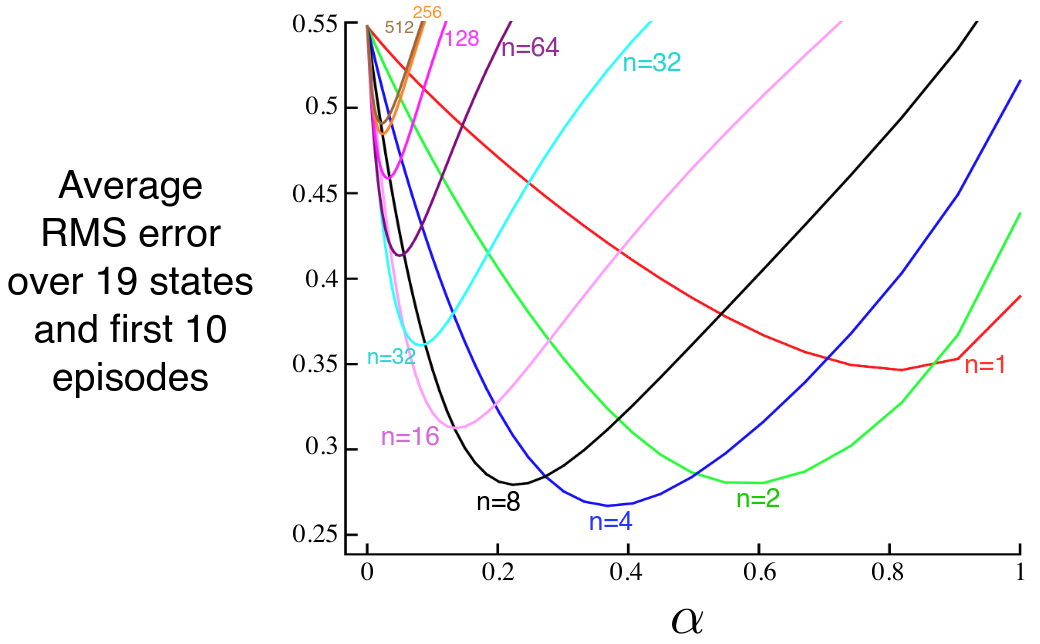
\includegraphics[width=0.8\textwidth]{images/n-step-comparison.png}
    \caption{Comparison between $n$-step methods as a function of $\alpha$ for various values of $n$ in a random-walk task. An intermediate value of $n=4$ performs best, converging faster than both TD methods ($n=1$), and  MC methods ($n=512$). Image taken from \cite{sutton-barto}.}
    \label{fig:n-step-comparison}
\end{figure}
It can be shown that all $n$-step TD methods converge to the correct value function $v_{\pi}$ under appropriate technical conditions. The $n$-step TD methods hence form a family of sound methods, with one-step TD methods and Monte Carlo methods as extreme members.\\\\
For control problems, we can generalize one-step TD methods to their respective $n$-step versions by defining the $n$-step return in terms of estimated action values.
\begin{equation}
    G_{t:t+n} = R_{t+1} + \gamma R_{t+2} + \dots + \gamma^{n-1} R_{t+n} + \gamma^n Q(S_{t+n}, A_{t+n})
    \label{n-step-return-Sarsa}
\end{equation}
The update rule of $n$-step Sarsa is then the following:
\begin{equation}
    Q(S_t, A_t) = Q(S_t, A_t) + \alpha (G_{t:t+n} - Q(S_t, A_t))
    \label{n-step-action-update}
\end{equation}
In essence, a new TD control algorithm can be constructed by incorporating a formula for the return into Equation \eqref{n-step-action-update}.\\
For example, we can define $n$-step Expected Sarsa by defining the $n$-step return in terms of the expected value of state $S_{t+n}$.
\begin{equation}
    G_{t:t+n} = R_{t+1} + \gamma R_{t+2} + \dots + \gamma^{n-1} R_{t+n} + \gamma^n \sum_a{Q(S_{t+n}, a) \pi(a | S_{t+n})}
    \label{n-step-return-expected-Sarsa}
\end{equation}
And $n$-step Q-learning by defining the $n$-step return in terms of the maximum value of state $S_{t+n}$.
\begin{equation}
    G_{t:t+n} = R_{t+1} + \gamma R_{t+2} + \dots + \gamma^{n-1} R_{t+n} + \gamma^n \max_a{Q(S_{t+n}, a)}
    \label{n-step-return-Q-learning}
\end{equation}

It can be shown that all $n$-step methods converge to the optimal value function if the leaning  and that the convergence rate is independent of $n$.

\section{Discussion}
In this chapter we introduced the main concepts of reinforcement learning, we saw that reinforcement learning is a framework for learning in sequential decision-making problems, where the agent interacts with the environment and learns to maximize its reward.\\
We then presented Monte Carlo methods, which are a class of algorithms that use the full return \eqref{return} to estimate the value function, and TD methods, which use the one-step return \eqref{return-recursive}. TD methods are usually better than MC methods because they can be applied to continuing tasks, and reduce the variance of the value estimate.\\
Finally, we discussed $n$-step methods, which estimate the value function using the $n$-step return formula \eqref{n-step-return}. These methods have been proven to converge to the correct value function $v_{\pi}$ under specific conditions and represent a family of reliable techniques, with one-step TD methods and Monte Carlo methods being their two ends of the spectrum.

    \blankpage
    \chapter{Policy Gradient Methods}
So far we focused on action-value methods, those methods learned the action-value function $q$ and used it to derive a policy. In this chapter, we will focus on methods that learn the policy directly, without consulting a value, or action-value function. The value function still has an important role as it's often used to learn the policy, however, it is not required for action selection. This class of methods is called policy gradient methods.\\\\
Policy gradient methods can be applied without function approximation. However, in this discussion, we will concentrate on the function approximation setting, where the policy is expressed as a function of the state $s$ and a vector of parameters $\vect{\theta}$, expressed as $\pi(a|s; \vect{\theta})$.\\\\
We start by proving some background on function approximation, particularly neural nets which will be used in all algorithms presented. Then, we will see the policy gradient theorem for the case of discrete action spaces. Finally, we explore more recent methods that are used in practice, such as TRPO and PPO.\\\\

\section{Function Approximation}
The methods discussed so far represent the action-value function $q(s, a)$ as a table and are thus called tabular methods. These methods have been shown to converge to an optimal policy under certain conditions, such as proper selection of the step-size $\alpha$ and the policy $\epsilon$ parameter. However, these methods can be impractical to use in certain scenarios, such as when the state space is extremely large (e.g. in the game of chess or Briscola) or when the state space is continuous. In these cases, function approximation must be used to represent the value function, action-value function, and policy.\\\\
Consider the problem of finding the value function corresponding to a policy $\pi$, thus far we implemented the update rule for the value function by moving $v(s)$ closer to the return $G_t$ which represents the target:
\begin{equation}
    v(s) = v(s) + \alpha (G_t - v(s))
    \label{eq:tabular-update}
\end{equation}
With function approximation, the idea is the same, moving the output closer to the target. But instead of moving the value of the table entry directly, we need to change the parameter vector $\vect{w}$.\\\\
In theory, we could use any method from the supervised learning literature to perform function approximation, however in practice neural networks are most commonly used, so we will focus on them here.\\
The way we usually find the best parameter vector in neural nets is by minimizing a loss function. The loss function measures how far the output of the function is from the target. A natural loss function for learning the value is the \textit{mean squared error loss} denoted as $\mathrm{MSE}$:
\begin{equation}
    \mathrm{MSE} = \frac{1}{2}(G_t - \hat{v}(S_t; \vect{w}))^2
    \label{eq:mse}
\end{equation}
where $G_t$ is the return, which represents the target and $\hat{v}(s; \vect{w})$ is the output of the function, which represents the prediction.\\\\
We can find the best parameter vector $\vect{w}$ in a number of ways, in neural nets the most commonly used is gradient descent, that is, we update the weights in the negative direction of the gradient. To do this we need the gradient of the loss function with respect to the parameter vector $\vect{w}$, which can be computed as follows:
\begin{equation}
    \nabla_{w} \mathrm{MSE} = \left( \hat{v}(S_t; \vect{w}) - G_t \right) \nabla_w \hat{v}(S_t; \vect{w})
    \label{eq:mse-gradient}
\end{equation}
Where $\nabla_w \hat{v}(s; \vect{w})$ is the gradient of the output of the function with respect to the parameter vector $\vect{w}$ and can be quickly found with automatic differentiation techniques.\\\\
In the derivation of the gradient \eqref{eq:mse-gradient} we assumed $\nabla_w G_t = 0$, this is true for the case of Monte Carlo methods, where $G_t = R_{t+1} + \gamma R_{t+2} + \dots + R_T$, but not for TD methods, where $G_t = R_{t+1} + \gamma \hat{v}(S_{t+1}; \vect{w})$. In this case the gradient is not a true-gradient but a semi-gradient, because we left out the $\nabla_w G_t = \gamma \nabla_w \hat{v}(S_{t+1}; \vect{w})$ term. However, it can be shown that semi-gradient methods have better convergence properties than true-gradient ones, in particular true-gradient methods even in the tabular case without function approximation  won't converge to the value function $v_{\pi}$ in stochastic environments, that represent the majority of RL tasks. The interested reader can find an example of this behavior in chapter 11.5 of the Sutton and Barto book \cite{sutton-barto}.\\\\

\subsection{Policy Approximation}
In policy gradient methods, the policy can be parameterized in any way, as long as it is differentiable with respect to the parameter vector $\vect{\theta}$. Approximating the policy directly has many advantages over approximating the action-value function:
\begin{itemize}
    \item The approximate policy can approach a deterministic policy, whereas with $\epsilon$-greedy action selection the policy always has a probability of selecting a random action.
    \item It enables the selection of actions with arbitrary probabilities, for example, in imperfect information games performing always the same action is not optimal, because the opponent can learn the player's strategy and exploit it. Think for example the game of poker, the best strategy isn't to always bluff or always check, but to do a mix of both so that the opponent can't predict the agent behavior.
    \item The action probabilities change smoothly with the parameter vector $\vect{\theta}$, whereas with $\epsilon$-greedy action selection the probability can change dramatically for a small change in $\vect{\theta}$.
    \item Stronger convergence guarantees are available for policy-gradient methods.
    \item 
\end{itemize}

\section{Policy Gradient Theorem}
To understand the policy gradient theorem, we need to first define a performance measure of a policy $\pi$ with respect to a parameter vector $\vect{\theta}$:
\begin{equation}
    J(\vect{\theta}) = v_{\pi_{\theta}}(s_0) = \sum_a \pi_{\theta}(a|s_0) q_{\pi_{\theta}}(s_0, a)
    \label{eq:performance-measure}
\end{equation}
Where $v_{\pi_{\theta}}$ represents the true value function for the policy $\pi_{\theta}$, determined by the parameter vector $\vect{\theta}$.\\\\
The problem with equation \ref{eq:performance-measure} is that its gradient depends also on the gradient of the action-value function $q_{\pi_{\theta}}$, because, as the policy changes also the action-value function changes. Fortunately its gradient can still be computed using the policy gradient theorem:
\begin{equation}
    \begin{split}
        \nabla_\theta J(\vect{\theta}) & \propto \sum_s \mu(s) \sum_a q_{\pi}(s, a) \nabla_{\theta}\pi_{\theta}(a|S_t)\\
        & = \mathbb{E}_{\pi_{\theta}} \bigg[\sum_a q_{\pi}(S_t, a) \nabla_{\theta}\pi_{\theta}(a|S_t) \bigg]
    \end{split}
    \label{eq:policy-gradient-theorem}
\end{equation}
Where $\mu(s)$ is the state distribution, which is unknown, but can be approximated by the empirical distribution of the states visited during the policy evaluation. The policy gradient theorem allows to estimate the gradient of the performance measure with respect to the policy parameter in a way that does not involve the derivative of the state distribution.
The policy gradient theorem gives an exact expression proportional to the gradient; all that is needed is some way of sampling
whose expectation equals or approximates this expression.\\
We can further simplify expression \eqref{eq:policy-gradient-theorem} by multiplying and dividing by $\pi_{\theta}(a|S_t)$:
\begin{equation}
    \mathbb{E}_{\pi_{\theta}} \bigg[\sum_a q_{\pi}(S_t, a) \nabla_{\theta}\pi_{\theta}(a|S_t) \bigg] = \mathbb{E}_{\pi_{\theta}} \bigg[q_{\pi}(S_t, A_t) \frac{\nabla_{\theta} \pi_{\theta}(A_t|S_t)}{\pi_{\theta}(A_t|S_t)} \bigg]
    \label{eq:single-action-policy-gradient}
\end{equation}
In the last expression we removed the sum over the actions, this the most commonly used form of the policy gradient theorem and allows the computation of the policy gradient even with continuous action spaces.

\section{REINFORCE}
REINFORCE estimates the action-value function $q_{\pi_{\theta}}(s, a)$ of the policy gradient (\ref{eq:single-action-policy-gradient}) using Monte Carlo to estimate $q_{\pi}(S_t, A_t)$.
\begin{equation}
    q_{\pi}(S_t, A_t) = \sum_{t'=t}^T \gamma^{t'-t} R_{t' + 1} = G_t
\end{equation}
Thus the update rule for the policy parameter vector $\vect{\theta}$ is:
\begin{equation}
    \theta_{t+1} = \theta_t + \alpha G_t \frac{\nabla_{\theta} \pi_{\theta}(A_t|S_t)}{\pi_{\theta}(A_t|S_t)}
    \label{eq:reinforce-update}
\end{equation}
The update increases the probability of actions proportional to the return and inversely proportional to the probability of the action. This makes sense because we move towards actions that lead to a higher return and perform a bigger update for actions with a lower probability, which are selected and hence updated less often.

\subsection{REINFORCE with Baseline}
The policy gradient theorem \eqref{eq:policy-gradient-theorem} can be generalized by adding a baseline function $b(s)$ to the action-value function without loss of generality:
\begin{equation}
    \begin{split}
        & \sum_s \mu(s) \sum_a (q_{\pi}(s, a) - b(s)) \nabla_{\theta}\pi_{\theta}(a|S_t) = \\
        & = \sum_s \mu(s) \sum_a (q_{\pi}(s, a)) \nabla_{\theta}\pi_{\theta}(a|S_t) - \sum_s \mu(s) b(s) \sum_a \nabla_{\theta}\pi_{\theta}(a|S_t)\\
        & = \nabla_{\theta} J(\vect{\theta}) - \sum_s \mu(s) b(s) \nabla_{\theta} \sum_a \pi_{\theta}(a|s)\\
        & = \nabla_{\theta} J(\vect{\theta})
    \end{split}
    \label{eq:policy-gradient-theorem-generalized}
\end{equation}
Where in the last step we used the fact that $\nabla_{\theta} \sum_a \pi_{\theta}(a|s) = 0$. The baseline function $b(s)$ can be any function of the state $s$ and is used to reduce the variance of the gradient estimator.\\
One natural choice for the baseline function is the value function $v_{\pi_{\theta}}(s)$, which gives the REINFORCE with baseline update:
\begin{equation}
    \theta_{t+1} = \theta_t + \alpha (G_t - b(S_t)) \frac{\nabla_{\theta} \pi_{\theta}(A_t|S_t)}{\pi_{\theta}(A_t|S_t)}
    \label{eq:reinforce-with-baseline-update}
\end{equation}
Where $\hat{v}_{\pi_{\theta}}(S_t)$ is an estimate of the value function $v_{\pi_{\theta}}(S_t)$, which is estimated with Monte Carlo.

\section{Actor-Critic Methods}
Actor-Critic methods merge policy gradient and temporal difference methods. The policy gradient is used to update the policy parameter vector $\vect{\theta}$ and TD-learning is used to update the value function $v_{\pi_{\theta}}(s)$. This introduces a bias in the policy gradient update, however it also reduces variance and hence accelerates learning.\\
One-step actor-critic methods updates the policy as following:
\begin{equation}
    \theta_{t+1} = \theta_t + \alpha (R_{t+1} + \gamma \hat{v}_{\pi_{\theta}}(S_{t+1}; \vect{w}) - \hat{v}_{\pi_{\theta}}(S_t; \vect{w})) \frac{\nabla_{\theta} \pi_{\theta}(A_t|S_t)}{\pi_{\theta}(A_t|S_t)}
    \label{eq:one-step-actor-critic-update}
\end{equation}
Which is similar to the REINFORCE with baseline update \eqref{eq:reinforce-with-baseline-update}, but uses the one-step TD target $G_{t:t+1} = R_{t+1} + \gamma \hat{v}(S_{t+1}; \vect{w})$ instead of the full return $G_t$.\\
At the same time the value function is updated using the TD error:
\begin{equation}
    \vect{w}_{t+1} = \vect{w}_t + \alpha (R_{t+1} + \gamma \hat{v}_{\pi_{\theta}}(S_{t+1}; \vect{w}) - \hat{v}_{\pi_{\theta}}(S_t; \vect{w})) \nabla_{\vect{w}} \hat{v}_{\pi_{\theta}}(S_t; \vect{w})
    \label{eq:one-step-actor-critic-value-function-update}
\end{equation}
These methods are called actor-critic methods because the policy is called the actor and the value function is called the critic. The critic learns the value function and the actor, given the value function, learns the policy.

\section{Trust Region Policy Optimization}
    \blankpage
    \chapter{Original work}

In this chapter we explain the approach that was used to create a reinforcement learning agent that learns to play Briscola. The code implementation is available at \url{https://github.com/LetteraUnica/BriscolaBot}.

\begin{figure}[H]
    \centering
    \includesvg[width=0.9\textwidth]{images/general-architecture.svg}
    \caption{Starting from the Agent Pool, 4 opponents with frozen parameters are sampled. If the pool contains fewer than 4 agents, sampling is continued with replacement. The agent then plays 512 games against each opponent, resulting in a total of 2048 games (corresponding to 40960 tricks), which are played in parallel using a Vectorized Environment. During episode generation, the agent also collects experience and stores it in an Experience Buffer. Afterwards, the agent is trained on the collected experience using the PPO algorithm \cite{schulman2017proximal}. Finally, a copy of the updated agent is inserted into the Agent Pool with frozen weights. The process is repeated until the agent reaches the desired performance.}
    \label{fig:general-architecture}
\end{figure}
The general architecture \ref{fig:general-architecture} is composed of four main components, described in their respective sections in more detail:
\begin{itemize}
    \item \textbf{Vectorized Environment:} Implements the Briscola environment and allows for parallel execution of multiple games.
    \item \textbf{Agent Pool:} Stores a pool of agents with frozen weights. The agents are sampled during training to play against the agent being trained.
    \item \textbf{Experience Buffer:} Stores the experience collected by the agent during gameplay.
    \item \textbf{Optimization:} The agent is trained on the experience collected during gameplay using the PPO algorithm \cite{schulman2017proximal}.
\end{itemize}
After outlining the general architecture, we will explain the training process for the Briscola agent, along with the hyperparameters employed and performance evaluation. Ultimately, we will showcase the effectiveness of our approach by pitting the latest iteration of our agent, BriscolaBot-v3, against human players. To that end, interested readers can access the game at \url{https://replit.com/@LorenzoCavuoti/BriscolaBot}.

\section{Environment implementation}
To implement the environment we followed the guidelines of the PettingZoo library, which is a Python library for conducting research in multiagent reinforcement learning \cite{pettingzoo}. It is similar to OpenAI Gym, but it is designed for multiagent environments. We aimed to optimize the speed of the environment implementation to maximize the time spent in the training loop and minimize the time spent on executing game logic.

\subsection{Agent observation}
The agent has access to various information during gameplay, including the cards played so far, the cards in its hand, the Briscola card, the card on the table (if present), as well as its and the opponent's score. This information is represented in a vector with 162 components, as detailed in Table \ref{tab:state}.

\begin{table}[H]
    \centering
    \begin{tabular}{c c c c} 
     \hline
     Feature & n. components \\
     \hline
        Cards played & 40 \\
        Cards in hand & 40 \\
        Briscola card & 40 \\
        Table card & 40 \\
        \hline
        Agent points & 1 \\
        Opponent points & 1 \\
        \hline
        Total & 162 \\
        \hline
    \end{tabular}

    \caption{Features used as input to the agent in Briscola. The first set of features consists of one-hot encoded vectors, with each element indicating a card. For example, if a card has been played, the corresponding element is set to 1, while if it hasn't, it's set to 0. The same goes for the cards in hand, the Briscola card, and the card thrown by the opponent. The last two features show the agent's and opponent's scores, normalized by the highest possible score in Briscola to keep them within the range [0, 1].}
    \label{tab:state}
\end{table}

\subsection{Reward structure}
The reward structure is a weighted combination of two elements: win or loss and points earned in each turn:
\begin{equation}
    R = \alpha R_\textrm{win} + (1 - \alpha) R_\textrm{points}
    \label{eq:reward-structure}
\end{equation}
The reward structure consists of two terms: $R_\textrm{win}$ and $R_\textrm{points}$. $R_\textrm{win}$ is equal to 1 if the agent wins the game and 0 otherwise, and is only given at the end of the game. On the other hand, $R_\textrm{points}$ are the points the agent gains in each turn normalized by the highest possible score in Briscola and are given at every turn. The relative importance of these two terms is controlled by $\alpha$, which is a hyperparameter. Ideally, $\alpha=1$ should give the best results as it prioritizes winning. However, this can also lead to high variance in the reward structure and sparse rewards, with only 0 or 1 being given at the end of the game. In practice, we started training with $\alpha=0.1$ and the gradually increased it until we reached $\alpha=1$. This allows to learn fast a the beginning of training and then focus on winning the game.

\subsection{Action space}
We explored two different ways to represent the action space. The first representation consisted of three discrete actions, corresponding to each of the three cards the agent could play, making it an intuitive choice that mimics how humans play the game. In this representation all actions are valid except when near to the end of the game, where the player has fewer than 3 cards in hand. The second representation consisted of 40 discrete actions, each representing a card from the deck. This representation is less intuitive and most of the actions, around 93\%, are invalid. Despite these limitations, the second representation outperformed the first (as shown in Figure \ref{fig:action-space-comparison}). We believe this is because the agent doesn't have to consider the position of the cards in its hand and can instead focus solely on the cards it holds.
\begin{figure}[H]
    \centering
    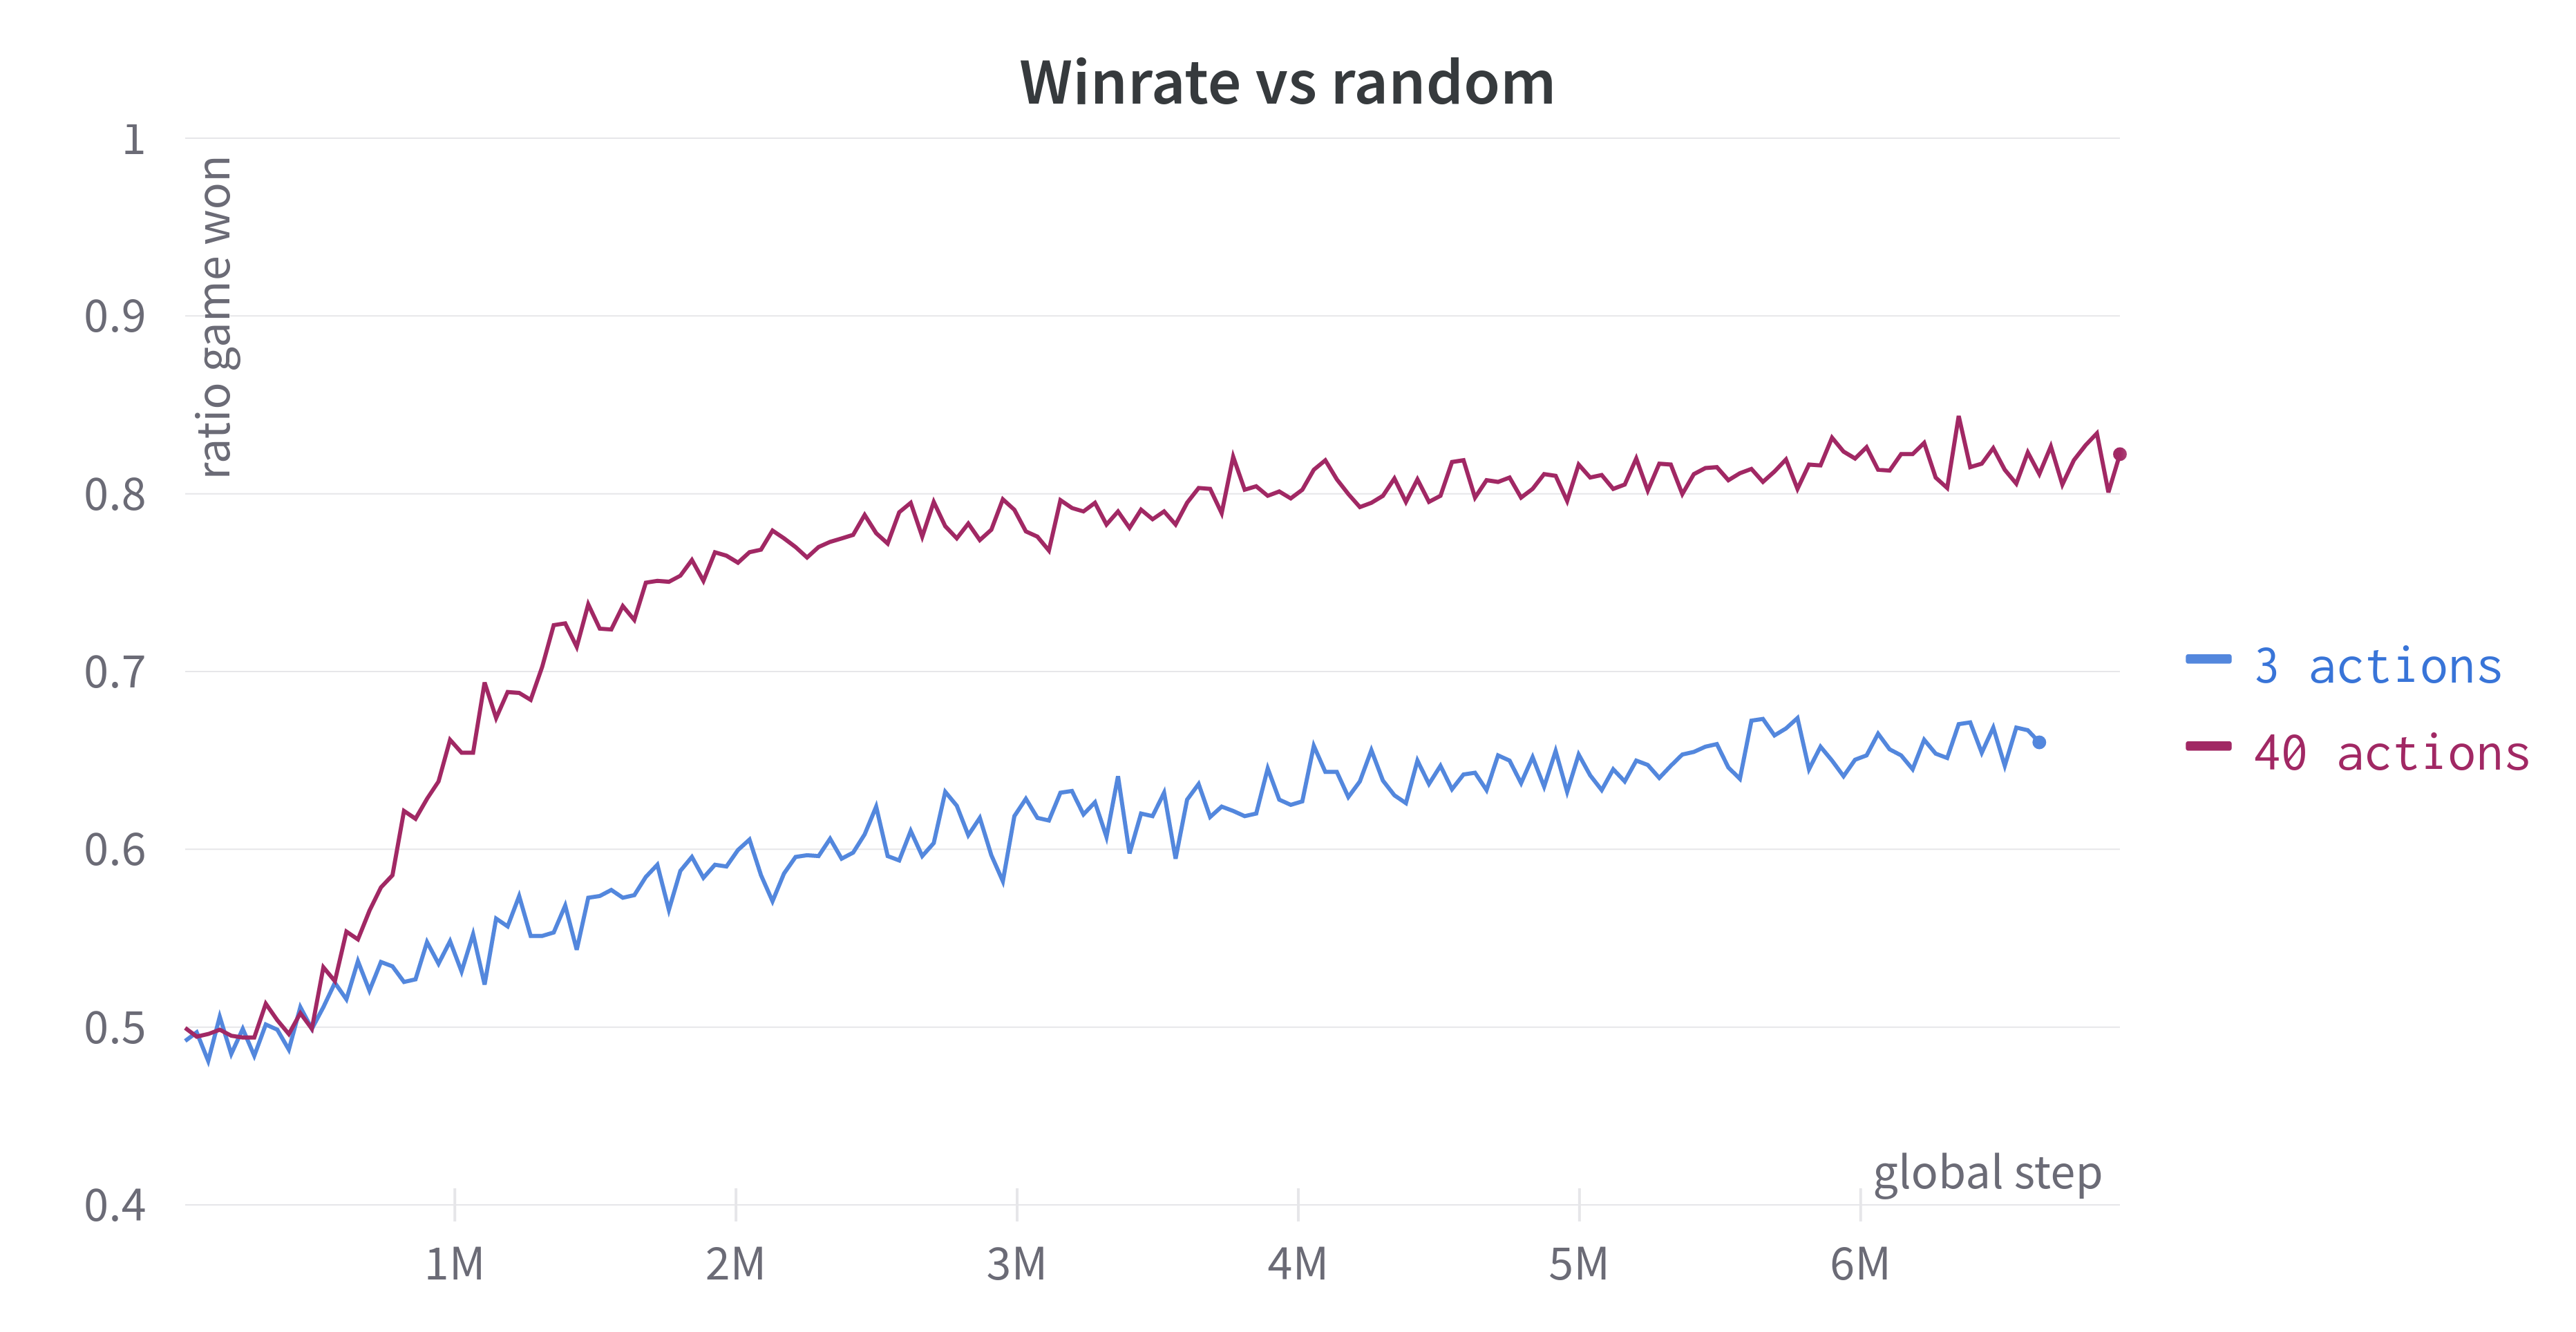
\includegraphics[width=\textwidth]{images/action-spaces-comparison.png}
    \caption{Performance of the two action space representations against a random player. The representation with 40 actions learns faster and reaches a win rate higher than 80\%, while the 3 action representation learns more slowly and reaches a win rate of 65\% by the end of training. In both representations we used invalid action masking as described in \cite{action-masking}.}
    \label{fig:action-space-comparison}
\end{figure}

\subsubsection{Invalid action masking}
Both in the first and second representation of the action space, the agent must not play a card that is not in its hand. This can be ensured through different methods, such as penalizing the agent for playing an invalid action or masking the invalid actions. We opted to implement the latter approach, as it has been shown empirically to be superior to penalizing invalid actions \cite{action-masking}.

The masking is done by setting the logits corresponding to the invalid actions to a small number, this way of performing the masking can be demonstrated to still produce a valid policy gradient as we are applying a differentiable state-dependent transformation to the policy \cite{action-masking}.

\begin{equation*}
    \pi'(\cdot|s) = \mathrm{softmax}(\mathrm{mask}(l_i))
\end{equation*}
\begin{equation*}
    \mathrm{mask}(l_{i}) = \begin{cases}
        l_i & \text{if $a_i$ is valid} \\
        M & \text{otherwise}
    \end{cases}
\end{equation*}
Where $l$ is the logits vector, $a$ is the action vector, $s$ is the state and $M$ is a small number, in our implementation we used $M=-10^6$.

\subsection{Vectorized environment}
In order to make the training process faster, we utilized a vectorized environment. This is a wrapper around the original environment that allows multiple instances of it to run simultaneously. In this setup, the agent receives all observations from all environments at once, which enables batching of policy evaluation and potentially performing it on a GPU, resulting in a significant speed-up of the training process.

\section{Agent}
When using policy-gradient methods the agent consists of two parts, the Actor and the Critic. The Actor, implemented as a multi-layer perceptron (MLP) with ReLU activations, defines the policy by mapping the agent's observation to a probability distribution over the action space (Figure \ref{fig:actor-critic-network}). On the other hand, the Critic uses the same MLP architecture as the Actor but outputs a single real value that represents the state's value (Figure \ref{fig:actor-critic-network}). We used two separate neural networks for the Actor and Critic as suggested in \cite{ppo-implementation-details}.

\begin{figure}[H]
    \centering
    \includesvg[width=0.6\textwidth]{images/actor-critic-net.svg}
    \caption{Diagram of the Actor-Critic Network Architecture. The Actor (left) transforms the agent's observation into a probability distribution over the 40 available actions, while the Critic (right) outputs a single real value, representing the state's value.}
    \label{fig:actor-critic-network}
\end{figure}

\section{Agent Pool}
The agent pool serves as a repository for past versions of the agent undergoing training, and keeps track of each version's win probability against the current agent. In detail, the pool holds a list of agents and their ratings $E_i$ against the agent being trained\footnote{The rating is very similar to the ELO system}. When opponents are selected for training, the pool samples them based on their ratings, with higher-rated agents having a higher probability of being chosen. This sampling is done using the following formula:

\begin{equation}
    P_i = \frac{e^{E_i}}{\sum_{j=1}^n e^{E_j}}
    \label{eq:agent-pool-sampling}
\end{equation}

The ratings of the opponents in the agent pool are updated after the agent has played games against them, with the following equation:

\begin{equation}
    E_i \rightarrow (1-\nu) E_i + \nu \, \textrm{logit}(\bar W_i)
    \label{eq:agent-pool-rating-update}
\end{equation}

Where $E_i$ represents the rating of opponent $i$, $\bar W_i$ is the average win rate of opponent $i$ against the agent being trained. The hyperparameter $\nu$ determines the influence of the old rating $E_i$ and the new rating $\textrm{logit}(\bar W_i)$ on the updated rating. If $\nu = 1$, the updated rating would be an unbiased estimator of the true rating. However, this would result in high variance. To reduce the variance, $\nu = 0.1$ is used, which biases the estimator towards $E_i$, reducing its variance.\\\\
The agent pool is a crucial component as it prevents the agent from forgetting how to overcome previous versions of itself. With the agent pool, the agent is exposed to a diverse range of opponents, including those it has previously defeated, and must be able to overcome them once again, thus ensuring its overall improvement.

\section{Optimization}
The optimization process is done using a variant of the Proximal Policy Optimization (PPO) algorithm, which includes several modifications that have been shown to improve the performance of the algorithm \cite{ppo-implementation-details}. Some of them are:
\begin{itemize}
    \item The learning rate decreases gradually during training, a common practice in deep learning that has been shown to also enhance PPO's performance.
    \item Generalized Advantage Estimation (GAE): The advantage function is calculated using GAE \cite{schulman2015high}, reducing variance in the advantage function and shortening training time.
    \item Normalization of Advantages: After GAE is used to calculate the advantages, they are normalized at the mini-batch level to have mean zero and unit variance. This operation doesn't change the policy gradient, but it helps the optimization process as the data is centered around zero.
    \item Loss entropy bonus: The loss function is enhanced with an entropy bonus, encouraging exploration and preventing the policy from becoming too deterministic too early in training.
\end{itemize}

The optimization of the agent is performed using the Adam optimizer \cite{kingma2014adam}, with a starting learning rate of $3 \cdot 10^{-3}$, which gradually decreases to $1 \cdot 10^{-4}$ during the training process. To accelerate training, a large batch size of 1024 to 2048 is employed, as it has been observed to increase efficiency, and it aligns with the typical use of large batch sizes in reinforcement learning \cite{mccandlish2018empirical}. The agent's performance is optimized by minimizing the following loss function.

\begin{equation}
    L = L_{\textrm{policy}} + \beta_\textrm{v} L_\textrm{value} - \beta_\textrm{e} L_\textrm{entropy}
    \label{eq:ppo-loss}
\end{equation}
In equation \eqref{eq:ppo-loss}, $L_{\textrm{policy}}$ represents the PPO policy loss as in equation \eqref{eq:ppo-update-clip}, $L_\textrm{value}$ is the mean squared error between the predicted value and the actual episode return, and $L_\textrm{entropy}$ is the entropy of the policy. The hyperparameters $\beta_\textrm{v}$ and $\beta_\textrm{e}$ control the relative importance of these terms and are commonly set around $0.5$ and $0.01$ respectively.

\section{Training Procedure}
We trained three agents with increasing level of performance using an incremental approach, similar to the one used when developing chess engines \cite{stockfish,lc0}. More in detail, when developing the next version of Stockfish, the developers measure its performance against the previous version, if the new version wins more games than the previous version, it is considered an improvement. This is a simple yet powerful approach as it allows to test the agent improvement without having to define an ELO rating, which can be hard to do, as it depends on the distribution of the opponents.

\subsection{BriscolaBot-v1}
The first version of the agent didn't use self-play with the agent pool, instead was only trained against a random opponent for 10 million steps. Before starting the final training run, however, we performed an extensive hyperparameter search using the Weights \& Biases bayesian search method \cite{wandb}. The algorithm was tasked to maximize the win probability against a random opponent in 1 million training steps. The method successfully discovered hyperparameters that reduced the time taken to reach an 80\% win rate against a random agent by half, as depicted in Figure \ref{fig:hyperparam-best-default}. The optimized hyperparameters are displayed in Table \ref{tab:hyperparam-best}.

\begin{figure}[H]
    \centering
    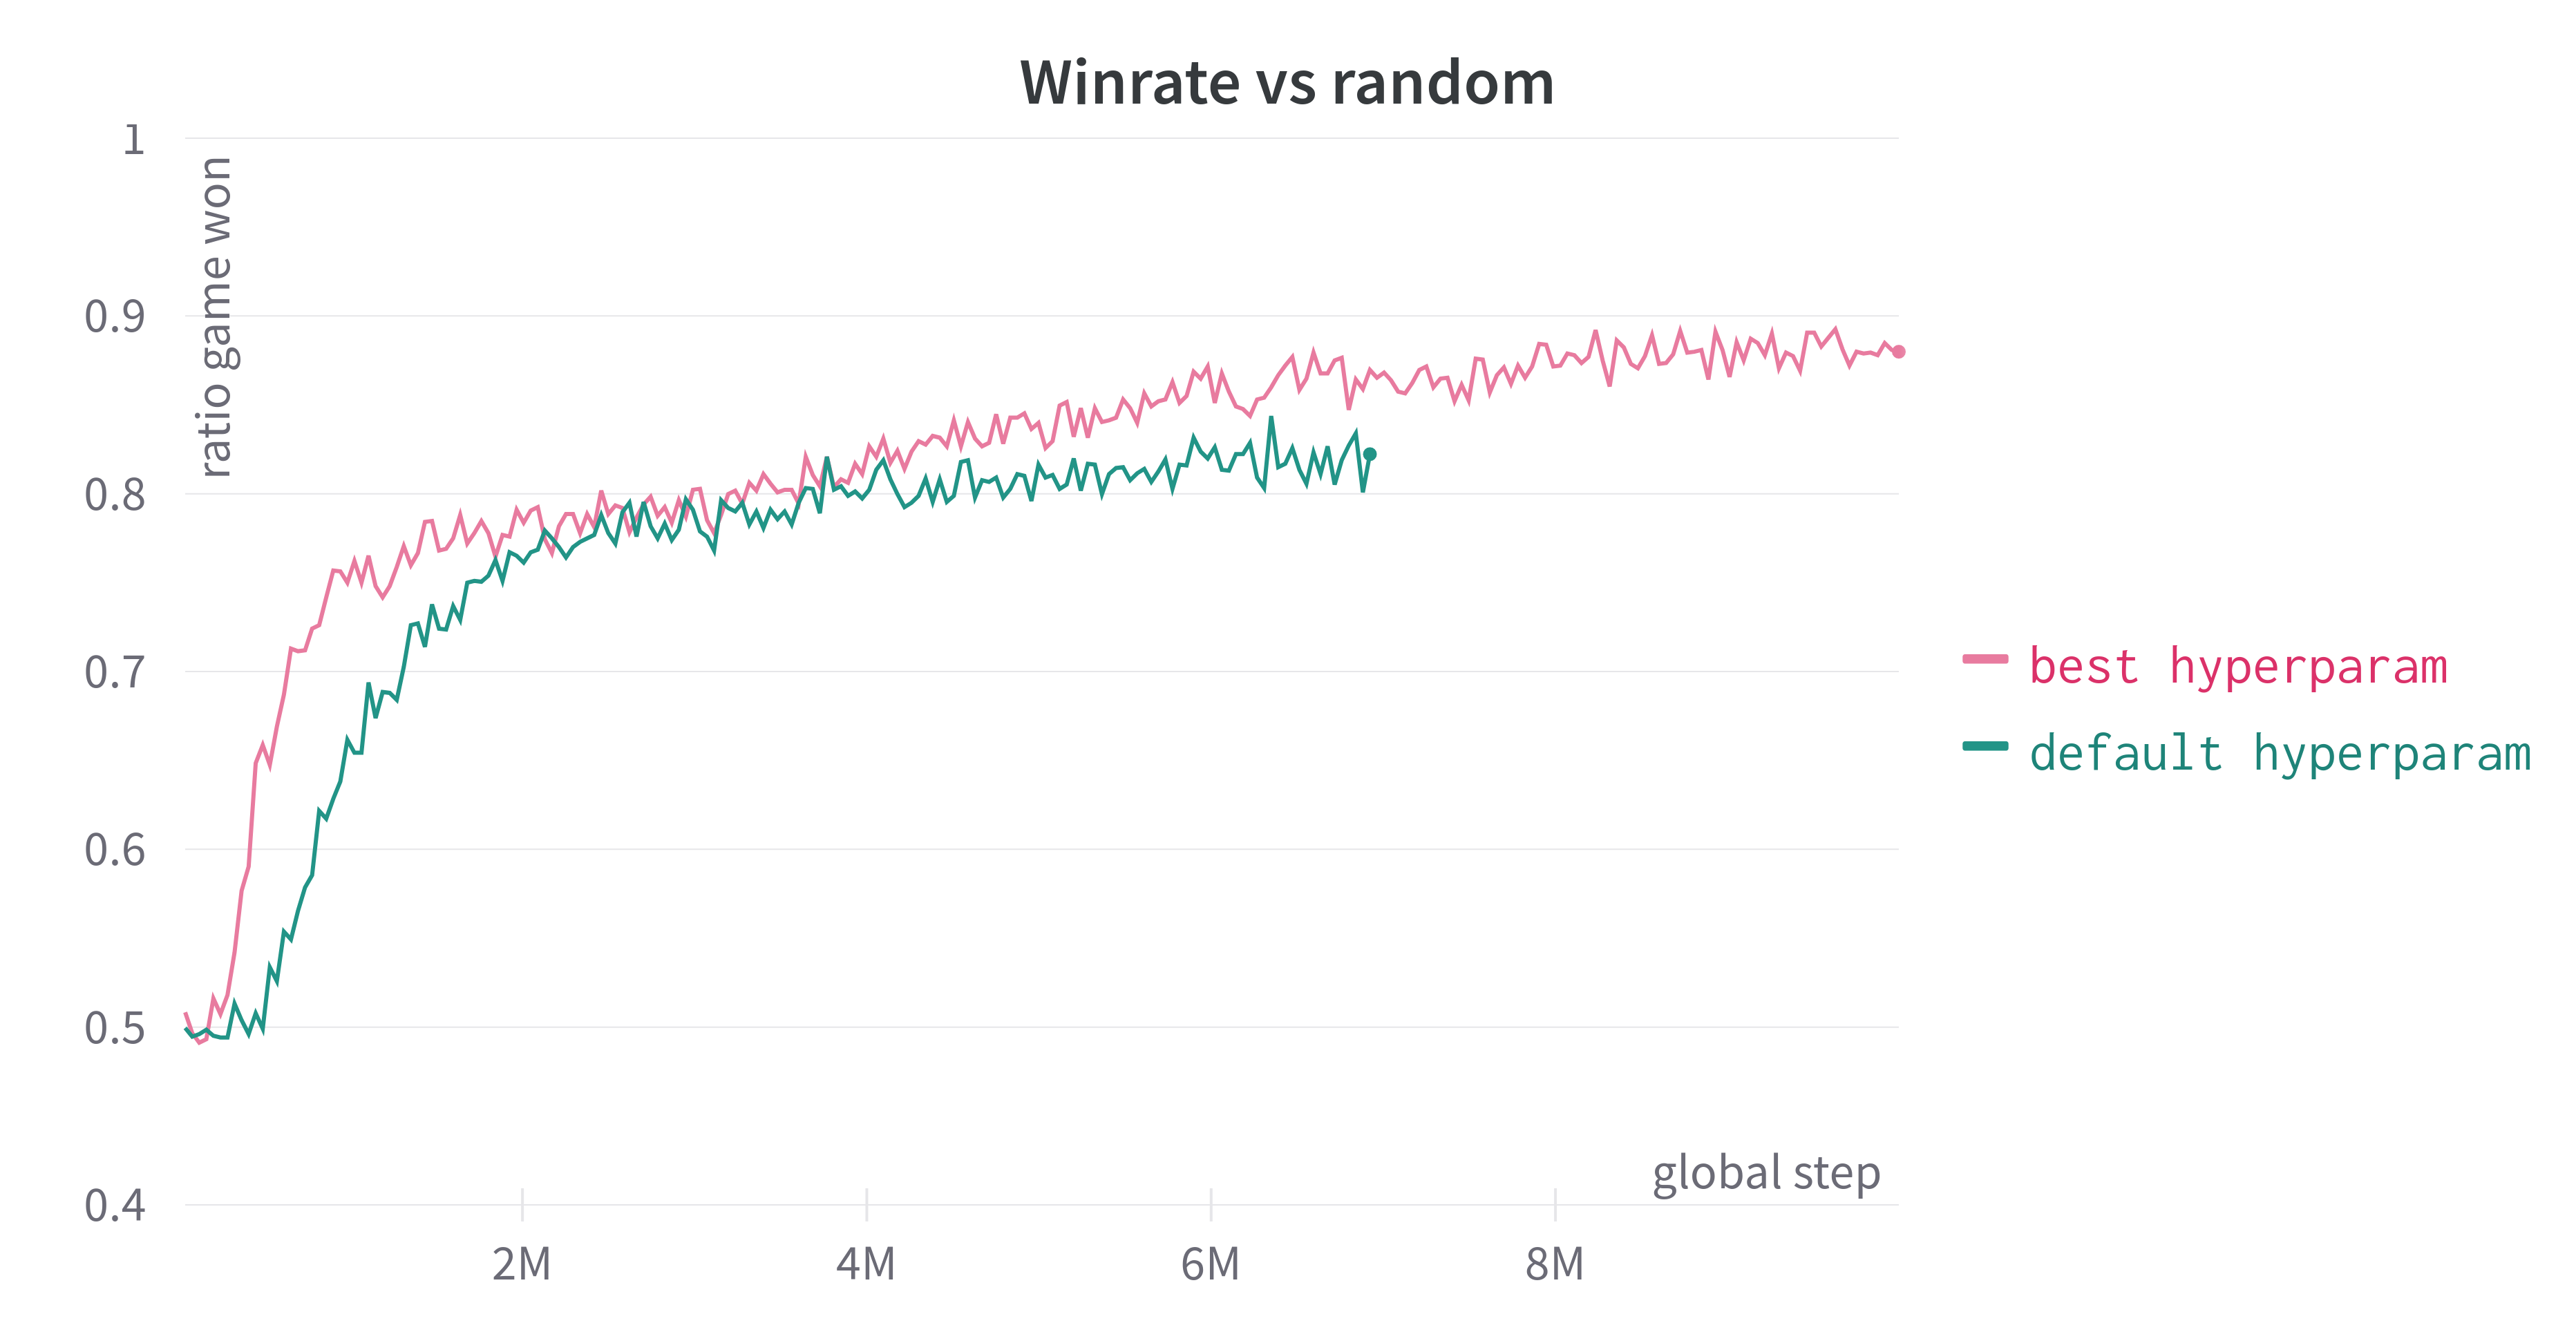
\includegraphics[width=\textwidth]{images/hyperparam-best-default.png}
    \caption{Comparison of the default hyperparameters and the best hyperparameters found using Weights \& Biases bayesian search method.}
    \label{fig:hyperparam-best-default}
\end{figure}

\begin{table}[H]
    \centering
    \begin{tabular}{ccc}
        \hline
        Hyperparameter & Default value & Best value \\
        \hline
        Learning rate & 0.001 & 0.003 \\
        Clip coefficient \eqref{eq:ppo-update-clip} & 0.2 & 0.3\\
        Entropy bonus \eqref{eq:ppo-loss} & 0.001 & 0.01 \\
        GAE $\lambda$ \eqref{eq:gae-advantage} & 0.95 & 0.9 \\
        Discount factor $\gamma$ \eqref{return-recursive} & 1 & 1 \\
        Ratio win reward \eqref{eq:reward-structure} & 0 & 0.1 \\
        Update epochs & 4 & 2 \\
    \end{tabular}
    \caption{Best hyperparameters found using Weights \& Biases bayesian search method. The default parameters were taken from the CleanRL implementation of PPO \cite{huang2022cleanrl} which provide a good starting point for reinforcement learning tasks. Update epochs is the number of passes over the collected episode data the optimization process performs.}
    \label{tab:hyperparam-best}
\end{table}

The final training run, which produced BriscolaBot-v1, was performed using the optimized hyperparameters. The agent was able to achieve a win rate of 80\% against a random agent in 1 million steps and almost 90\% in 10 million steps, as shown in figure \ref{fig:hyperparam-best-default}.

\subsection{BriscolaBot-v2}
In the second version of the agent, we added self-play with the agent pool, because the agent manages beat a random opponent very quickly. Furthermore, we increased the neural network size to 256, changed the activation function from ReLU to Mish \cite{misra2019mish} and added learning-rate decay. The effect of some of these changes can be seen in figure \ref{fig:mish-activation}. With these changes the new agent was able to beat BriscolaBot-v1 60\% of the time when trained for 10 million steps, which is a very good result considering the randomness of the game of Briscola.

\begin{figure}[H]
    \centering
    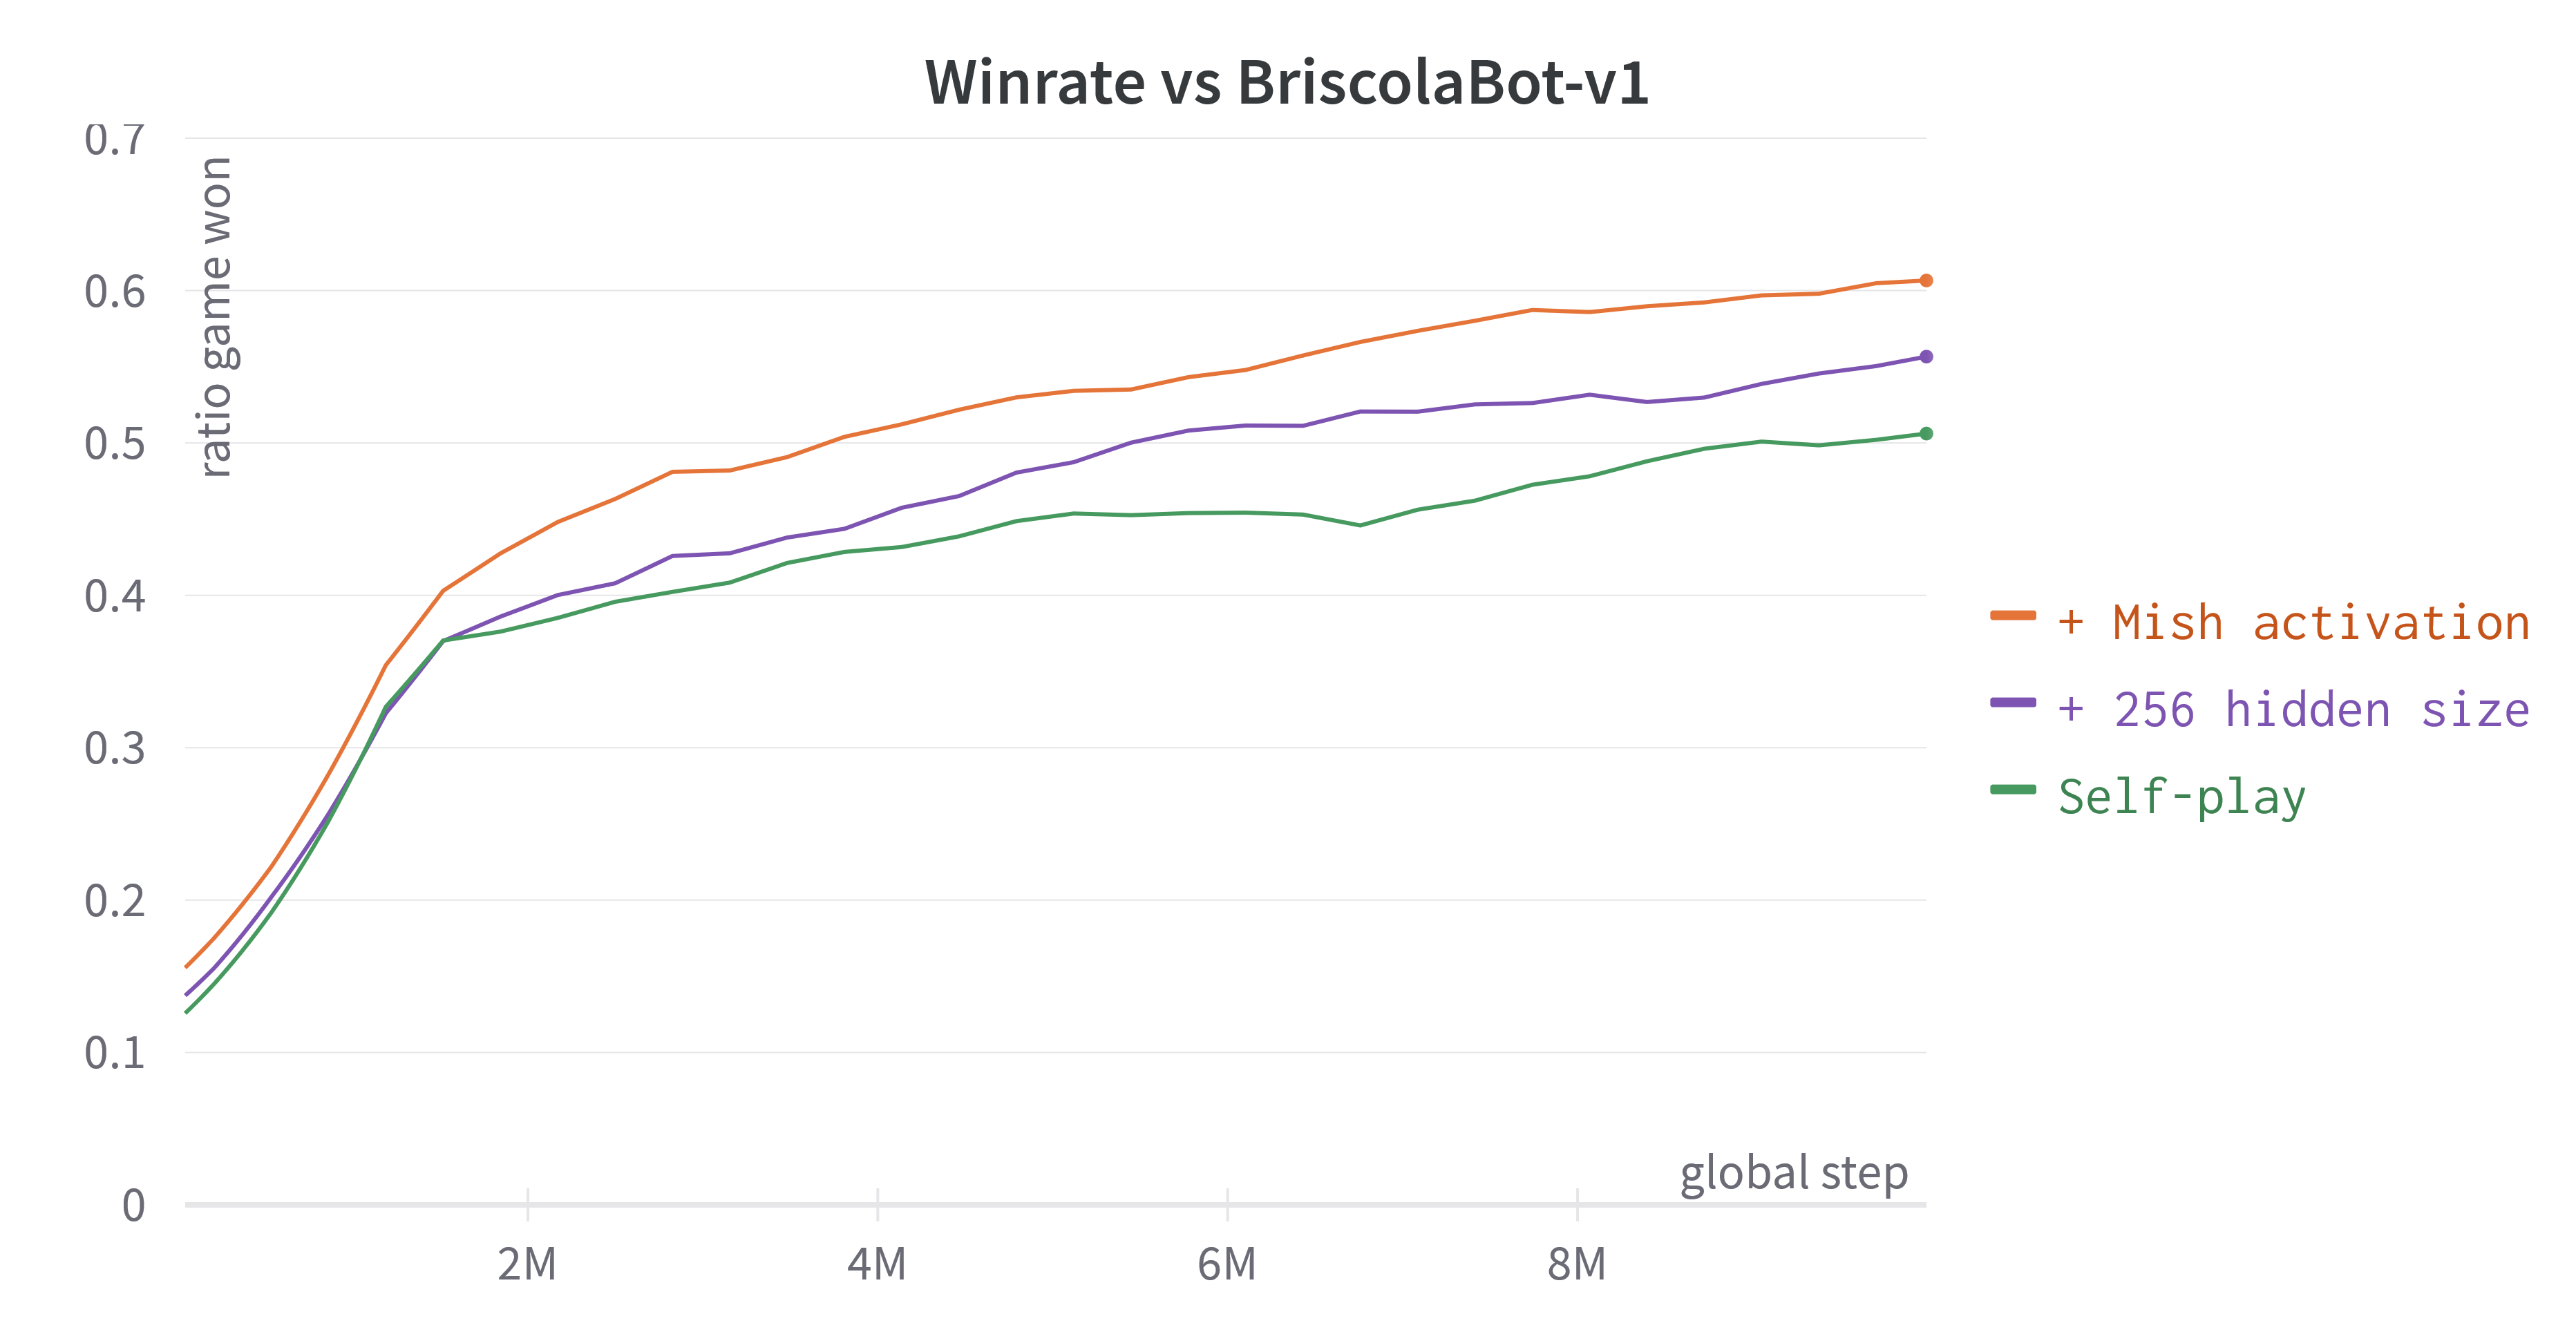
\includegraphics[width=\textwidth]{images/mish-activation.png}
    \caption{Winrate against BriscolaBot-v1 when increasing the neural network size from 128 to 256 (purple line) and on top of that changing the activation function from ReLU to Mish (orange line).}
    \label{fig:mish-activation}
\end{figure}

To produce the final version of the BriscolaBot-v2 agent we continued training until 20 million steps. BriscolaBot-v2 was able to achieve a win rate of 90\% against a random agent and 64\% against BriscolaBot-v1.

\subsection{BriscolaBot-v3}
A problem with BriscolaBot-v2 is that it throws the ace and the 3 of briscola very often, instead of waiting for the right opportunity. This is a problem, because the ace and the 3 of briscola are the most powerful cards in the game, and wasting them can lead to a loss.\\\\
We think that this problem is caused by giving too much importance to the number of points scored in the loss function, which, combined with $\gamma = 0.95$ causes the agent to collect points as soon as possible. In this version, we tried to address this problem by gradually increasing the $\nu$ parameter in equation \eqref{eq:reward-structure} from 0.1 up to 1 during training. Another change that we applied was to decay the entropy $\beta_\textrm{e}$ parameter in equation \eqref{eq:ppo-loss} from 0.01 down to approximately zero, as this is an exploration parameter and should decrease when reaching optimal play \cite{open-ai-five}. The effect of these changes can be seen in figure \ref{fig:briscolabot-v3}.

\begin{figure}[H]
    \centering
    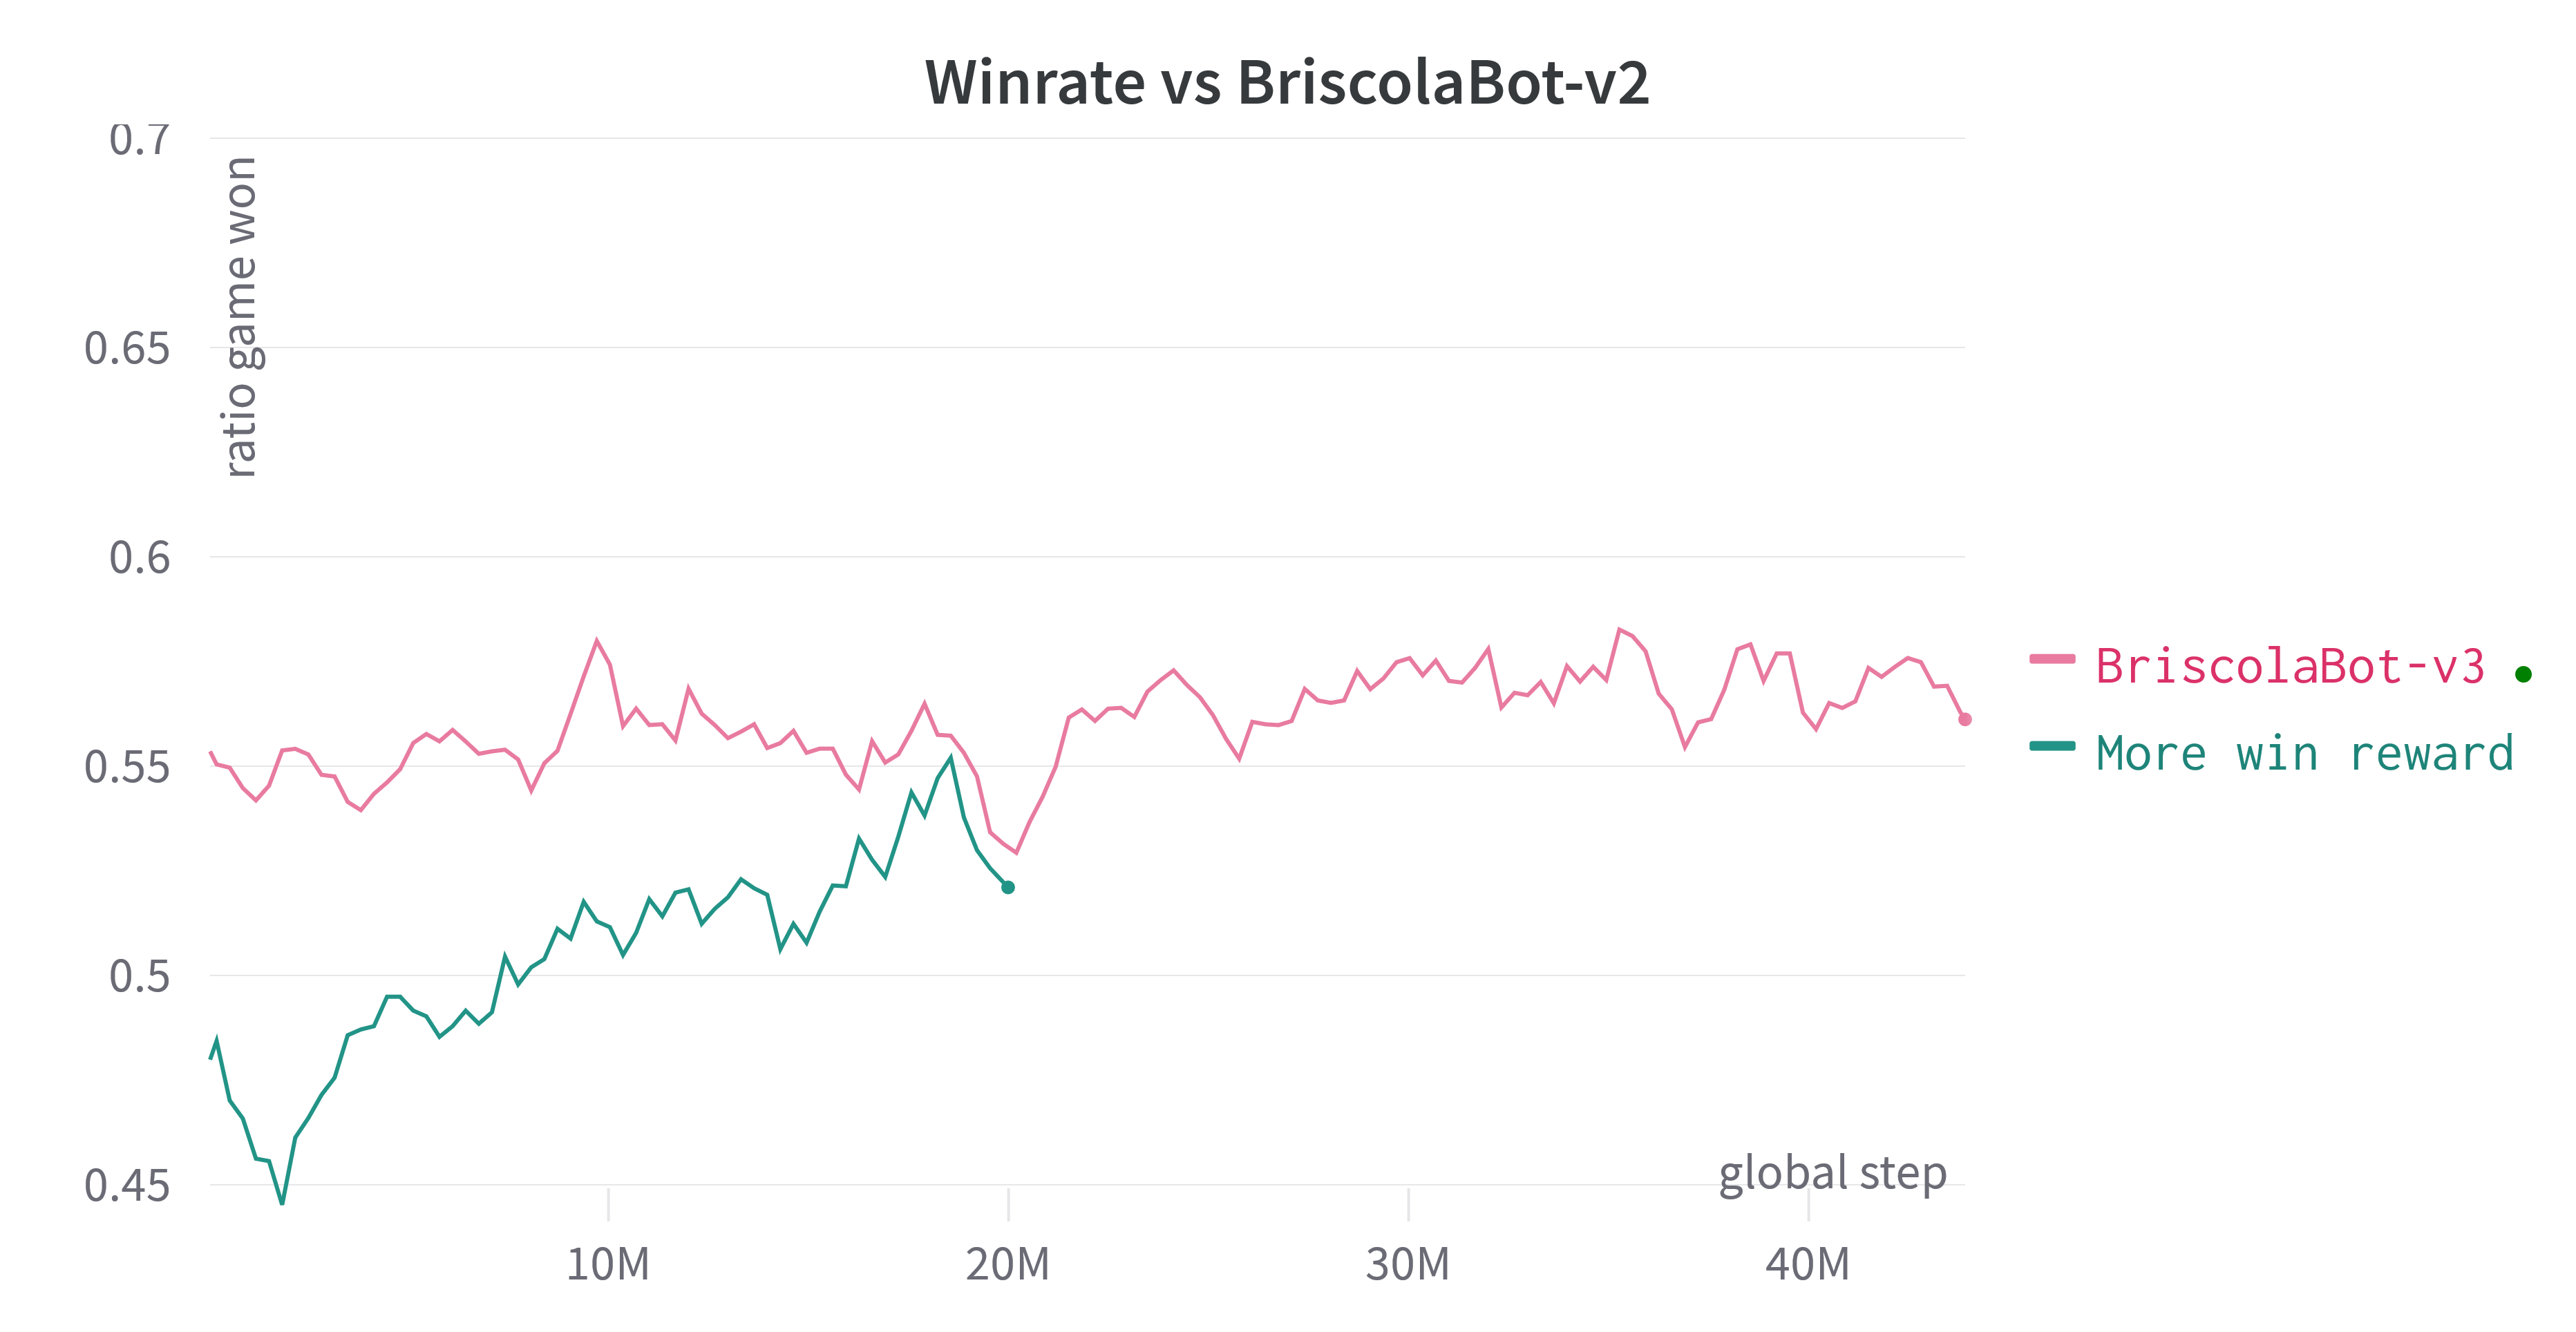
\includegraphics[width=\textwidth]{images/briscolabot-v3.png}
    \caption{Winrate against BriscolaBot-v2 when gradually increasing the $\nu$ parameter in equation \eqref{eq:reward-structure} and decreasing the entropy during training, we can see that these two changes improved the performance of the agent. Since these two runs started from the weights of BriscolaBot-v2, the ratio of games won starts near 0.5.}
    \label{fig:briscolabot-v3}
\end{figure}

The final agent was trained starting from the BriscolaBot-v2 weights, with the modifications listed above for 50 million steps, corresponding to approximately 4 hours of training on an intel i5-4690K CPU. The agent was able to achieve a win rate of 57\% against BriscolaBot-v2 and 93\% against a random agent, surpassing previous approaches to the problem \cite{alsora-deep-briscola-dqn}. The final list of hyperparameters used for the final agent is shown in Table \ref{tab:hyperparam-final}.

\begin{table}[H]
    \centering
    \begin{tabular}{cccc}
        \hline
        Hyperparameter & Value & Hyperparameter & Value \\
        \hline
        Learning rate & 0.003 & Learning rate decay & 0.997 \\
        Clip coefficient & 0.3 & Batch size & 2048 \\
        Discount factor $\gamma$ & 1 & GAE $\lambda$ \eqref{eq:gae-advantage} & 0.9 \\
        Entropy bonus $\beta_\textrm{e}$ \eqref{eq:ppo-loss} & 0.01 & $\beta_\textrm{e}$ decay & 0.998 \\
        Ratio win reward $\nu$ \eqref{eq:reward-structure} & 0.1 & $\nu$ increase & 0.001 \\
        Update epochs & 2 & hidden layer size & 256
    \end{tabular}
    \caption{Hyperparameters used for the final agent. We decay or increase the parameters every 2048 games played, corresponding to 40960 steps.}
    \label{tab:hyperparam-final}
\end{table}

\section{Human evaluation}
We evaluated the performance of BriscolaBot-v3 by having human players play against it using our website, available at \url{https://replit.com/@LorenzoCavuoti/BriscolaBot}. The human evaluation results are presented in Table \ref{tab:human-evaluation}.\\

\begin{table}[H]
    \centering
    \begin{tabular}{cccccc}
        \hline
        Opponent & Games played & Won & Lost & Win probability & 90\% CI\\
        \hline
        Me & 16 & 6 & 10 & 0.38 & 0.21-0.58\\
        Alessandro & 17 & 5 & 12 & 0.52 & 0.16-0.50\\
        Daniel & 10 & 2 & 8 & 0.2 & 0.08-0.47\\
        Giacomo & 10 & 4 & 8 & 0.2 & 0.14-0.51\\
        Silvio & 23 & 12 & 11 & 0.52 & 0.36-0.68\\
        Simone & 39 & 19 & 20 & 0.49 & 0.36-0.62\\
        Teresa & 13 & 6 & 7 & 0.46 & 0.26-0.67\\
        Others & 10 & 3 & 7 & 0.3 & 0.14-0.56\\

        \hline
        \textbf{Total} & 142 & 57 & 85 & 0.4 & 0.34-0.47\\
    \end{tabular}
    \caption{Results of the human evaluation study. The Won and Lost columns represent the games won and lost by the human against the BriscolaBot-v3 agent. The confidence interval (CI) is calculated exactly using the Beta distribution and reflects the degree of uncertainty around the estimated win rate. The agent is shown to win about 60\% of the games against human players, with a 90\% confidence interval of 0.53 to 0.66.}
    \label{tab:human-evaluation}
\end{table}
The human evaluation study demonstrates the strength of our agent, where it has \textbf{won against human players 60\% of the time}, with a 90\% confidence interval of 0.53 to 0.66.\\
All the human players we tested against expressed that the agent is very good at the game. One of the best performing players, Simone, found the agent frustrating to play against because it seemed to predict his hand cards, as the agent sometimes threw a briscola when he had a hand full of aces and threes of different seeds than briscola.\\\\
Despite its success, the agent can still be improved, as it occasionally makes suboptimal moves. For instance, it can throw the 7 of briscola instead of taking the trick with the 4 of briscola, which would have allowed it to save the 7 for later use. Probably the agent has't learned these minor optimizations because they provide minimal gains in terms of points.

    \blankpage
    \chapter{Discussion}
In this thesis, we proposed a novel approach to solving the game of Briscola by using the PPO algorithm with function approximation to learn the optimal policy. To evaluate the performance of our latest agent, BriscolaBot-v3, we developed a website, accessible at \url{https://replit.com/@LorenzoCavuoti/BriscolaBot}, where the agent could play against human players. Our results showed that BriscolaBot-v3 achieved a 60\% win rate, with a 90\% confidence interval of [0.53, 0.66], against average human players, confirming the effectiveness of our method. Moreover, the agent was trained on a standard 4-core computer, ensuring reproducibility of our results and making it feasible to train a competitive agent on any machine in a reasonable amount of time.

\section{Future Work}
We have identified several potential improvements to further enhance the performance of the agent, including:
\begin{itemize}
    \item \textbf{Exact solving of endgame positions:} when all cards have been extracted the cards of the opponent are known, so it becomes possible to solve the game of Briscola exactly with minimax search. This improvement can be achieved at a low computational cost, since the number of possible ways of playing out a given endgame is only 36, which can be further reduced through the application of dynamic programming techniques.
    \item \textbf{Improve agent performance with MCTS:} previous methods in the game of Briscola used Monte Carlo Tree Search (MCTS) to identify the best move \cite{Briscola-mcts-Playing-Algorithm, villa2013-briscola-mcts}. However, these approaches relied on a model of the opponent rather than learning from it, such as assuming the opponent throws a random card from the set of unseen cards. We suggest improving this approach by training a model that predicts the opponent's possible move in a given situation, which can then be used to perform MCTS search.
    \item \textbf{Approximating the Nash equilibrium:} we can use imperfect information game-solving approaches to directly find or approximate the Nash equilibrium of the game of Briscola. These approaches have been used successfully in poker to beat the world's best players \cite{libratus}.
    \item \textbf{Extend the observation space of the agent:} currently, the agent only observes the cards that have been played, but not the order in which they were played. By observing the order in which cards were played, the agent could potentially better predict the cards that the opponent has in their hand. For example, if the agent plays an ace of cups and the opponent does not use briscola to take the trick, it is likely that the opponent does not have any briscola in their hand. This information could allow the agent to be more aggressive in the following tricks.
\end{itemize}
Possible other directions for future work include applying the same technique to other Italian card games, such as Scopa, Tressette, Macchiavelli, and Scala 40. Additionally, the approach can be extended to Briscola when played with multiple players, as the game can be played by up to six players in teams of two or three.

    \printbibliography
\end{document}